%!TEX root = ../thesis.tex
%*******************************************************************************
%*********************************** Second Chapter *****************************
%*******************************************************************************

\chapter{Statistical aspects}  \label{c:2}

\ifpdf
\graphicspath{{Chapter2/Figs/pdf/}}
\else
\graphicspath{{Chapter2/Figs/svg/}}
\fi

\epigraph{`I often say that when you can measure what you are speaking about, and express it in numbers, you know something about it; but when you cannot measure it, when you cannot express it in numbers, your knowledge is of a meagre and unsatisfactory kind; it may be the beginning of knowledge, but you have scarcely, in your thoughts, advanced to the stage of \textit{science}, whatever the matter may be.'}{W. \citet{Kelvin1889}}

\section{Analysing the blood methylome to study human ageing}

\smallskip

\subsection{Building a DNA methylation dataset from public data}

\smallskip

During the last years large amounts of DNA methylation data have been generated to study complex diseases and ageing \citep{Rakyan2011,Flanagan2015}. Many of these datasets can be obtained from public repositories, such as the NCBI-hosted Gene Expression Omnibus (\acrshort{GEO}) \citep{Edgar2002}. Given its clinical accessibility and ease of collection, blood is one of the most commonly profiled tissues in human DNA methylation studies \citep{Flanagan2015}, including published studies on developmental disorders \citep{Aref-Eshghi2018} (see Chapter~\ref{c:3}). Therefore, I decided to use blood as my surrogate tissue to broaden our understanding of the human epigenetic ageing clock.

\bigskip

Furthermore, most of these human datasets have been generated using different versions of the Illumina Infinium array technology, with the Illumina Infinium HumanMethylation450 array (450K) being the most frequently used platform \citep{Flanagan2015}. Additionally, given that the different array versions have different chemistries, biases and number of probes \citep{Bibikova2009,Bibikova2011,Pidsley2016}, I decided to focus on 450K data for my analyses. Using the \textit{GEOquery} R package \citep{Davis2007}, I programmatically downloaded from GEO all the DNA methylation data from human blood that I could find, including samples from both whole blood and peripheral blood mononuclear cells (\acrshort{PBMC}). Furthermore, the data also had to satisfy the following criteria:

\begin{itemize}
	
	\item Raw DNA methylation data was available (i.e. IDAT files). This was required so the pre-processing pipeline and the batch effect correction (which requires access to control probes intensities, see section~\ref{s:2.2.3}) could be consistently applied across all the samples in the study.
	
	\item Metadata for the samples was available, with the chronological age as a minimum requirement. 
	
	\item In order to study physiological ageing, the blood samples were collected from individuals without prior disease diagnoses. However, it is important to mention that I could never be completely certain of this, since there could be a lack of diagnosis and/or lack of reporting of the disease in the metadata. 
	
\end{itemize}

\smallskip

This allowed me to assemble a \textbf{human blood DNA methylation dataset for healthy individuals} (after \acrshort{QC}, total $N=2218$) with the characteristics shown in Table~\ref{table:c2_table1}, which spans the entire human lifespan (0.5 to 101 years). Fig.~\ref{fig:c2_fig1} shows that the chronological age distribution is bimodal, with peaks around 10.69 and 58.81 years respectively. This reflects a sampling bias in human population studies, with more data being generated for the periods of postnatal development and during the appearance of age-related disease. However, in order to understand the development of complex diseases as a consequence of the ageing process, efforts should be made to also sample people in their middle ages, before the diseases are normally diagnosed.   


\begin{table}
%\centering
\small
	\begin{tabular}{ p{2cm} p{1cm} p{1cm} p{1cm} p{2cm} p{6cm} }
		\toprule
		\textbf{Batch name} & \textbf{N$_{\female}$} & \textbf{N$_{\male}$} & \textbf{N} & \textbf{Median age (years)} & \textbf{Other comments} \\
		\midrule
		Europe & 0 & 121 & 121 & 10.96 & - \\
		Feb\_2016 & 0 & 1 & 1 & 0.50 & - \\
		GSE104812 & 19 & 29 & 48 & 9.00 & - \\
		GSE111629 & 111 & 124 & 235 &  71.00 & - \\
		GSE40279 & 336 & 314 & 650 & 65.00 & - \\
		GSE41273 & 0 & 51 & 51 & 10.25 & - \\
		GSE42861 & 239 & 96 & 335 & 55.00 & - \\
		GSE51032 & 253 & 78 & 331 & 54.57 & Only people that remained cancer-free in the follow-up after sample collection were included  \\
		GSE55491 & 1 & 5 & 6 & 29.50 & - \\
		GSE59065 & 49 & 46 & 95 & 34.00 & - \\
		GSE61496 & 72 & 78 & 150 & 57.00 & Only one member of each twins pair was included \\
		GSE74432 & 29 & 22 & 51 & 12.00 & - \\
		GSE81961 & 25 & 0 & 25 & 30.05 & - \\
		GSE97362 & 39 & 80 & 119 & 13.00 & - \\
		\midrule
		\textbf{Total} & 1173 & 1045 & 2218 & 55.00 & - \\ 
		\bottomrule
	\end{tabular}
	\vspace*{3mm}
	\caption[Overview of the blood DNA methylation dataset from healthy individuals]{Overview of the blood DNA methylation dataset from healthy individuals (control). All the batches were downloaded from GEO \citep{Edgar2002}, with the exception of `Europe' and `Feb\_2016', which were generated in-house by my collaborators in Canada (see Chapter~\ref{c:3}). $N_{\female}$: number of samples from females. $N_{\male}$: number of samples from males. $N$: total number of samples. These numbers correspond to the samples left after applying quality control (QC, see section~\ref{s:2.1.2}).}
	\label{table:c2_table1}
\end{table} 


\begin{figure}[htbp!] 
	\centering    
	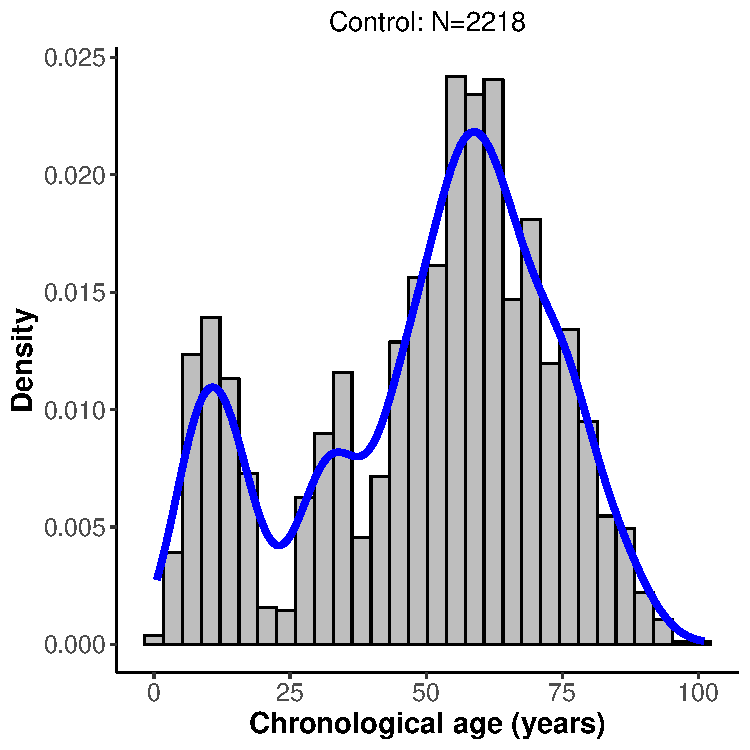
\includegraphics[width=0.6\textwidth]{C2_Fig1}
	\vspace*{2mm}
	\caption[Chronological age distribution in the healthy individuals]{Histogram showing the chronological age distribution for all the healthy individuals included in the DNA methylation dataset. The blue line represents the 1D kernel density estimate, as calculated by the \textit{stat\_density} function in R with default parameters.}
	\label{fig:c2_fig1}
\end{figure}

\smallskip

\subsection{Main DNA methylation data pre-processing pipeline} \label{s:2.1.2}

\smallskip

The analysis of DNA methylation data generated in Illumina arrays has been a topic of huge discussion and statistical innovation in the epigenetic community. There are plenty of reviews in the literature that discuss the different steps that should be involved in the pre-processing of this data type \citep{Wilhelm-Benartzi2013,Morris2015,Liu2016}. More specifically, a recent study by Je Liu and Kimberly D. Siegmund systematically benchmarked the pre-processing methods available for the 450K array in order to reduce variation among technical replicates and improve the detection of biological differences \citep{Liu2016}. Inspired by their results, I implemented a pre-processing pipeline for the 450K data using the \textit{minfi} R package \citep{Aryee2014} embedded in the following steps (Fig.~\ref{fig:c2_fig2}):

\begin{enumerate}
	
	
	\item \textbf{Background correction}. I used the \textit{noob} method \citep{TricheJr2013}, as implemented in the \textit{preprocessNoob} function from the \textit{minfi} R package \citep{Aryee2014}. \textit{noob} allows accounting for technical variation in the background (i.e. non-specific) fluorescence signal, which can lead to a reduced dynamic range for the methylation values ($\beta$-values) obtained (Fig.~\ref{fig:c2_fig2}b, Fig.~\ref{fig:sc2_fig1}) \citep{TricheJr2013}. Briefly, when measuring fluorescence intensities in the Illumina array platforms, the observed intensity (also known as foreground, $X_f$) is composed of:
	
	\begin{align}
	X_f = X_s + X_b
	\end{align}
	
	where $X_s$ is the true signal and $X_b$ is the background signal. Making use of a normal-exponential convolution (which assumes $X_s\sim Exp(\gamma)$ and $X_b\sim N(\mu, \sigma^2)$) and the `out-of-band' (\acrshort{OOB}) intensities (fluorescence signals in the opposite colour channel in Infinium I probes) to model $X_b$ , \textit{noob} is capable of estimating $X_s$ given $X_f$. Furthermore, I also applied the default dye-bias correction strategy, which controls for the different average intensities in the two colour channels \citep{TricheJr2013}. 
	
		\item \textbf{Quality control} (QC). Following guidelines from the \textit{minfi} R package \citep{Aryee2014}, I kept only those samples that satisfied the following criteria:
		
		\begin{enumerate}
			
			\item The sex predicted from the DNA methylation data (\acrshort{Sexp}) was the same as the reported sex in the metadata. The sex was predicted  using the \textit{getSex} function from the \textit{minfi} R package \citep{Aryee2014}, which employs intensity information from the sex chromosomes, such that:
			
			\begin{align}
			\text{Sex}_{p} = 
			\begin{cases}
			\text{female, } &\text{if: } (\mathrm{median}\left\{\log_2(M_{y}+U_{y})\right\} -  \mathrm{median}\left\{\log_2(M_{x}+U_{x})\right\}) < c \\
			\text{male, } &\text{if: } (\mathrm{median}\left\{\log_2(M_{y}+U_{y})\right\} -  \mathrm{median}\left\{\log_2(M_{x}+U_{x})\right\}) \geq c \\
			\end{cases}
			\end{align}
			
			where $M_{y}$ and $U_{y}$ represent the methylated and unmethylated intensity measurements for the array probes in the Y chromosome, $M_{x}$ and $U_{x}$ represent the methylated and unmethylated intensity measurements for the array probes in the X chromosome and $c$ is a predefined cutoff (default in \textit{minfi}: $c=-2$). A total of 13 samples (0.56\%) did not satisfy this criterion.
			
			\smallskip
			
			\item They were not outliers according to their global intensity values after background correction, such that:
			
			\begin{align}
			\frac{\mathrm{median}\left\{\log_2(M_{i})\right\} + \mathrm{median}\left\{\log_2(U_{i})\right\}}{2} \geq 10.5
			\end{align}
			
			where $M_{i}$ and $U_{i}$ represent the background-corrected methylated and unmethylated intensity measurements for all the 450K array probes (Fig.~\ref{fig:sc2_fig2}). A total of 95 samples (4.09\%) did not satisfy this criterion. 
			
		\end{enumerate} 
	
	\item \textbf{Probe filtering}. I filtered out the following types of probes:
	
	\begin{itemize}
		
		\item Probes that contain \acrshort{SNP}s at the single base extension site (position 0) or at the proximal CpG on the probe (positions 1-2), using the \textit{dropLociWithSnps} function in the \textit{minfi} package \citep{Aryee2014}. 
		
		\item Cross-reactive probes, as defined by \citet{Chen2013}. These are probes that can co-hybridise to alternative genomic sequences that are highly homologous to the target sequences \citep{Chen2013}.  
		
		\item  Probes that map to the sex chromosomes (X and Y).
	
	\end{itemize}
	
	It is important to mention that other authors have also filtered out probes with high detection p-value or low bead counts across samples \citep{Wilhelm-Benartzi2013,Morris2015}. However, I did not include these filters since it was not pointed out in the \textit{minfi} guidelines \citep{Aryee2014,Fortin2015} and it could complicate further downstream analyses (e.g. different sets of probes missing across different batches).     
	
	
	\begin{figure}[htbp!] 
		\centering    
		\includegraphics[width=0.8\textwidth]{C2_Fig2}
		\vspace*{2mm}
		\caption[Main DNA methylation data pre-processing pipeline]{Main DNA methylation data pre-processing pipeline. \textbf{a.} Flowchart showing the main steps implemented to pre-process the DNA methylation data from the 450K methylation arrays. The number of samples (N$_{\text{samples}}$) and the number of array probes (N$_{\text{probes}}$) left after each step are also specified for the samples from the healthy individuals. \textbf{b.}  $\beta$-value distributions, calculated using the raw fluorescence intensities (i.e. before any pre-processing), for the samples in the GSE41273 batch. Each curve represents a different sample. In grey: 51 samples that passed quality control (QC). In red: 2 samples that failed QC.  \textbf{c.} As in b., but calculating the $\beta$-values after background correction. \textbf{d.} As in b., but calculating the $\beta$-values after background correction, QC, probe filtering and BMIQ normalisation (i.e. the final $\beta$-values that I used for downstream analyses). Note that the samples that failed QC have been removed.}
		\label{fig:c2_fig2}
	\end{figure}
	
	
	\item \textbf{$\beta$-value calculation}. The methylation status of a given cytosine (normally found in a CpG site) in one of the array probes can be quantified using the $\beta$-value statistic, which is calculated as \citep{Wilhelm-Benartzi2013,Du2010}:
	
	\begin{align}
	\beta_i = \frac{\text{max}(M_i,0)}{\text{max}(M_i,0) + \text{max}(U_i,0) + \alpha}
	\end{align}
	
	where $M_i$ and $U_i$ represent the methylated and unmethylated intensity measurements for the $i$th-probe and $\alpha$ is a constant offset (in this work $\alpha = 100$, as recommended by Illumina) \citep{Du2010}. 
	
	In a DNA molecule of a single cell, a specific cytosine is either unmethylated or methylated (categorical / binary variable). However, given that a bulk DNA sample from a tissue is composed of thousands of cells (which can include different cell types with different methylation patterns), $\beta$-values result in a continuous variable between 0 and 1. A value of 0 means that all the measured DNA molecules are unmethylated ($0\%$) and a value of 1 means that all the measured DNA molecules are methylated ($100\%$) in that cytosine, which is roughly equivalent to say that 100\% of the cells are either unmethylated or methylated respectively in that cytosine for the sampled tissue. The $\beta$-values for a given sample (i.e. considering all the cytosines measured) usually follow a bimodal distribution, where the two peaks are centred around 0 and 1 (Fig.~\ref{fig:c2_fig2}d). 
	
	Other authors have used M-values to quantify methylation levels in arrays (Fig.~\ref{fig:sc2_fig3}), which can be calculated as:
	
	\begin{align}
	\text{M-value}_i = \log_2 \left(\frac{\text{max}(M_i,0) + \alpha}{\text{max}(U_i,0) + \alpha}\right)
	\end{align}
	
	with a default offset value of $\alpha=1$.  Du \textit{et al.} reported that $\beta$-values suffer from severe heteroscedasticity (i.e. differences in the variance) for highly methylated or unmethylated CpG sites and therefore the M-values have more desirable statistical properties \citep{Du2010}. However, Zhuang \textit{et al.} later showed that this only becomes a problem in studies with small sample sizes \citep{Zhuang2012} (which is not the case for my analyses). Furthermore, $\beta$-values are easier to interpret biologically and can be readily used in the context of BMIQ normalisation (see below). For these reasons, I choose $\beta$-values as the main methylation variable for this work.
	
	\item \textbf{Beta-mixture quantile normalisation} (\acrshort{BMIQ}). In the case of the 450K arrays two types of probes / chemistry coexist in the same platform. Infinium I probes and Infinium II probes have different $\beta$-values distributions (a.k.a. Infinium II probe bias). BMIQ is an intra-array normalisation strategy that allows to correct for this bias and has been shown to outperform other methods used in this context \citep{Teschendorff2012,Dedeurwaerder2011,Touleimat2012,Maksimovic2012}. BMIQ fits a three-state beta-mixture model to Infinium I and Infinium II probes separately and then maps the Infinium II probes distribution into the Infinium I probe distribution (Fig.~\ref{fig:c2_fig3}). In the case of unmethylated ($\beta$-values close to 0) and methylated ($\beta$-values close to 1) probes, this is done by transforming probabilities into quantiles. In the case of `hemimethylated' probes (intermediate $\beta$-values), a dilation transformation is applied to preserve the monotonicity and continuity of the data \citep{Teschendorff2012}. I applied BMIQ to my samples and discarded those that failed the normalisation step.  
	
\end{enumerate}

 
\begin{figure}[htbp!] 
	\centering    
	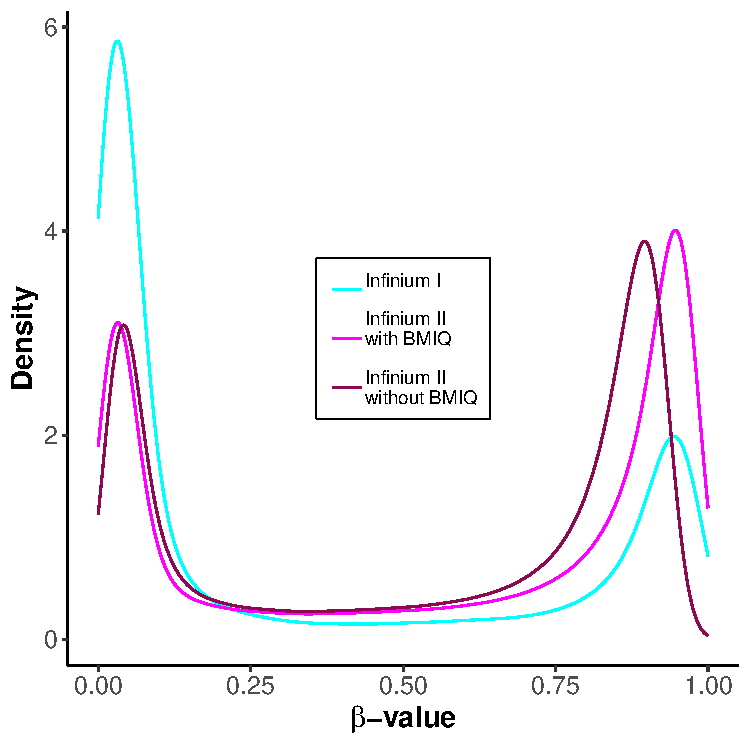
\includegraphics[width=0.8\textwidth]{C2_Fig3}
	\caption[Effect of BMIQ normalisation on the $\beta$-value distribution]{Effect of BMIQ normalisation on the $\beta$-value distribution of different subsets of array probes with different chemistries (Infinium I, Infinium II). These results correspond to a DNA methylation sample from the GSE41273 batch. It can be appreciated how BMIQ transforms the distribution of the Infinium II probes into a distribution more similar to the Infinium I probes.}
	\label{fig:c2_fig3}
\end{figure}

\smallskip

\subsection{Accounting for blood cell composition changes during ageing} \label{s:2.1.3}

\smallskip

Whole blood is composed of several cell types that contain a nucleus, including neutrophils, eosinophils, basophils, CD14$^+$ monocytes, CD4$^+$ T cells, CD8$^+$ T cells, CD19$^+$ B cells and CD56$^+$ natural killer (\acrshort{NK}) cells \citep{Teschendorff2017}. These cell types have different epigenetic profiles and, as a consequence, changes in their proportions (i.e. changes in blood cell composition) can affect bulk DNA methylation measurements \citep{Reinius2012}.

\bigskip

Accounting for this cellular heterogeneity is really important in epigenome-wide association studies (\acrshort{EWAS}) \citep{Liu2013,Jaffe2014,McGregor2016}. Furthermore, previous research has highlighted changes in blood cell composition with age, which could be one of the causes behind immunosenescence \citep{Czesnikiewicz-Guzik2008,Kuranda2011,Chen2016a,Seidler2010,Manser2016}. Therefore, considering blood cell composition in the context of ageing-related studies and the epigenetic clock is fundamental in order to make sure that the observed age-related changes in the methylome are not a direct consequence of the changes in blood cell composition during ageing \citep{Chen2016,Horvath2016,Jaffe2014}.

\bigskip

Several methods have been developed to estimate the cell composition of a blood sample given a bulk DNA methylation measurement (a.k.a. cell-type deconvolution) \citep{Teschendorff2017,Titus2017,Teschendorff2017a,Teschendorff2018}. These methods can be broadly split in two categories:

\begin{itemize}
	
	\item \textbf{Reference-based approaches}. They use a pre-defined set of DNA methylation reference profiles for the cell types that are supposed to be present in the tissue. In the case of methylation arrays, these reference profiles can be constituted by the $\beta$-values for a subset of array probes that are highly discriminative of the underlying cell types. Assuming that the blood sample is a weighted linear sum of the $C$ reference profiles, the objective of the method is to find these weights ($w_c$), which should be equivalent to the actual cell type proportions (given the assumption $\sum_{c=1}^{C} w_c \leq 1$) \citep{Teschendorff2017}. In mathematical terms:
	
	\begin{align}
	\mathbf{y} = \sum_{c=1}^{C} w_c \mathbf{b_c} + \epsilon
	\end{align}
	
	where $\mathbf{y}$ is the DNA methylation profile of the sample being considered, $C$ is the number of underlying cell types, $\mathbf{b_c}$ is the DNA methylation profile for the $c$th cell type and $\epsilon$ is the error \citep{Teschendorff2017a}. Different algorithms have been applied to estimate the values of $w_c$, with the approach by \citet{Houseman2012} (which uses a linear constrained projection)  being the most widely used. 
	
	\item \textbf{Reference-free approaches}. Instead of making use of reference profiles for the cell types of interest, these methods generally calculate latent variables that capture variation driven by cell type composition, although the strategy and assumptions to derive these latent variables from the DNA methylation data is highly method-specific \citep{Teschendorff2017}. These methods become particularly useful when no references are available for the cell types that constitute the tissue \citep{Teschendorff2017}.
	
\end{itemize} 

However, reference-free approaches rarely provide estimates for the specific cell types in a given sample \citep{Teschendorff2017} (which are needed in the current modelling framework of the epigenetic clock) and they often rely on the assumption that the top components of variation correlate with cell composition \citep{Teschendorff2017a}, something that is not always true (especially in the case of developmental disorders, see Chapter~\ref{c:3}), Thus, I decided to benchmark different reference-based cell-type deconvolution strategies in blood. In this context I tested (Fig.~\ref{fig:sc2_fig4}):

\begin{itemize}
	
	\item \textbf{Different blood references}. As pointed out before, the quality of the reference, containing the DNA methylation profiles of the cell types to be inferred, is crucial \citep{Teschendorff2017a,Koestler2016}. The reference must be composed of those CpG sites (in this case, array probes) that are able to better discriminate between the different cell types. In my case I considered six major blood `cell types' for the inference: granulocytes (`\acrshort{Gran}'), CD4$^+$ T cells (`\acrshort{CD4T}'), CD8$^+$ T cells (`\acrshort{CD8T}'), CD19$^+$ B cells (`\acrshort{B}'), CD14$^+$ monocytes (`\acrshort{Mono}') and  CD56$^+$ natural killer cells (`\acrshort{NK}'). It is important to point out that granulocytes are not themselves a `biological cell type' (since they are composed of neutrophils, eosinophils and basophils), but will be considered as a single `computational cell type' as previously done \citep{Chen2016,Horvath2016}. I tested three different blood references whose constitutive probes were selected using different strategies:
	
	\begin{enumerate}
		
		\item The reference implemented in the \textit{estimateCellCounts} function from the \textit{minfi} R package \citep{Aryee2014}, which is widely used in the epigenetic literature. The reference probes were selected using $t$-statistics, by finding those probes that were differentially methylated in each cell type when compared with the rest of the cell types. Among those probes that showed differences at p-value $< 10^{-8}$, the 100 most differentially methylated probes by effect size (50 hypermethylated and 50 hypomethylated) were chosen for each cell type (making a total of 600 probes for the reference) \citep{Jaffe2014}. 
		
		\smallskip
		
		\item The reference implemented in the \textit{EpiDISH} R package (\textit{centDHSbloodDMC.m}) \citep{Teschendorff2017b}. The reference probes (\acrshort{DHS-DMCs}, 333 in total) were selected by leveraging information of both differentially methylated cytosines (\acrshort{DMCs}, using moderated $t$-statistics) and chromatin accessibility (DNase Hypersensitive Sites or \acrshort{DHS}) for each cell type \citep{Teschendorff2017a}.  
		
		\item The reference implemented as part of the \acrshort{IDOL} strategy (IDentifying Optimal DNA methylation Libraries) \citep{Koestler2016}. In this case, the reference probes (300 in total) were originally selected based on differential methylation criteria and are updated in an iterative manner, with the probability of being selected based on their contribution to prediction accuracy \citep{Koestler2016}.
	
	\end{enumerate}
	
	  The three references were built using the dataset from \citet{Reinius2012} (GSE35069), which I obtained directly from the \textit{FlowSorted.Blood.450k} R package \citep{Jaffe2018}. This dataset contains DNA methylation data generated in the 450K array for the six cell types considered, all of which were isolated using flow cytometry \citep{Reinius2012}. The $\beta$-values for the selected probes were averaged across the biological replicates for each cell type. 
	
	\item \textbf{Different DNA methylation pre-processing pipelines}. I tested different configurations for the pre-processing of both the gold-standard (see below) and the reference data. For example, I tested whether probe filtering according to the criteria outlined in the previous section (section~\ref{s:2.1.2}) is desirable, since this leads to the removal of some of the probes originally selected for the reference in the original publications \citep{Teschendorff2017a,Koestler2016} (Fig.~\ref{fig:sc2_fig4}). Furthermore, I also tested whether the prediction benefits from a similar pre-processing of both the gold-standard (or the dataset where the prediction will be made) and the reference.
		
	\item \textbf{Different deconvolution algorithms}. I tested the performance of the following algorithms: CP/QP (constrained projection/quadratic programming, originally implemented by \citet{Houseman2012}), RPC (robust partial correlations) \citep{Teschendorff2017a} and CIBERSORT (which was originally developed for cell-type deconvolution using RNA expression data) \citep{Teschendorff2017a,Newman2015}. One of the key differences between the algorithms is how the normalisation constrain ($\sum_{c=1}^{C} w_c \leq 1$) is implemented \citep{Teschendorff2017a}. All the algorithms were run using the implementations in the \textit{epidish} function from the \textit{EpiDISH} R package \citep{Teschendorff2017b}, with the exception of the run in the \textit{minfi} reference, for which I used the \textit{estimateCellCounts} function with default parameters for the 450K array \citep{Aryee2014}. 

\end{itemize}

In order to compare the results from the predictions against real cell composition values, I used a \textbf{gold-standard} dataset (GSE77797) containing 12 samples where known proportions of DNA isolated from the different blood cell types were mixed \citep{Koestler2016}. I assessed the accuracy of the predictions using three different metrics:

\begin{itemize}
	
	\item Root mean squared error ($RMSE$), which is calculated as (for a given cell type $c$):
	
	\begin{align}
	RMSE_c = \sqrt{\frac{\sum_{n=1}^{N} (\hat{y}_{cn} - y_{cn})^2}{N}}
	\end{align}
	
	where $\hat{y}_{cn}$ is the predicted proportion of the $c$th cell type in the $n$th sample, $y_{cn}$ is the real proportion of the $c$th cell type in the $n$th sample and $N$ is the total number of samples in the gold-standard dataset ($N=12$). A perfect prediction for a cell type would minimise the value of $RMSE_c$ (i.e. $RMSE_c = 0$).
	
	\item Mean absolute error ($MAE$), which is calculated as (for a given cell type $c$):
	
	\begin{align}
	MAE_c = \frac{\sum_{n=1}^{N} |\hat{y}_{cn} - y_{cn}|}{N}
	\end{align}
	
	A perfect prediction for a cell type would minimise the value of $MAE_c$ (i.e. $MAE_c = 0$).
	
	\item Coefficient of determination (R$^2$), which is calculated as (for a given cell type $c$):
	
	\begin{align}
	R^2_c = \frac{\sum_{n=1}^{N} (\hat{y}_{cn} - \bar{y}_c)^2}{\sum_{i=1}^{N} (y_{cn} - \bar{y}_c)^2}
	\end{align}
	
	where $\bar{y}_c = \frac{\sum_{n=1}^{N} y_{cn}}{N}$. A perfect prediction would maximise the value of $R^2_c$ (i.e. $R^2_c=1$).
	
\end{itemize}


The most accurate strategy, according to the $RMSE$ (mean across cell types: $1.9270$) and $MAE$ (mean across cell types: $1.5498$), is `\textbf{idol\_NFB\_houseman}' (Fig.~\ref{fig:c2_fig4}, Fig.~\ref{fig:sc2_fig5}) i.e. the strategy that uses the IDOL reference, with all the pre-processing steps from my main pipeline for both reference and gold-standard (\textit{noob} background correction, probe filtering and BMIQ normalisation) and employs Houseman's CP/CQ algorithm (Fig.~\ref{fig:sc2_fig4}). This strategy performed well in all the cell types (Fig.~\ref{fig:c2_fig5}) and I selected it for my cell-type deconvolution analyses. 

\bigskip

It is important to mention that the gold-standard dataset was generated as part of the same study where the IDOL reference was also derived \citep{Koestler2016}. However, the gold-standard samples were used as an independent validation of the IDOL reference and should not influence the conclusions of the benchmarking that I performed. In the future, it will be interesting to validate these conclusions using new gold-standard datasets generated from whole blood.

\bigskip


\begin{figure}[htbp!] 
	\centering    
	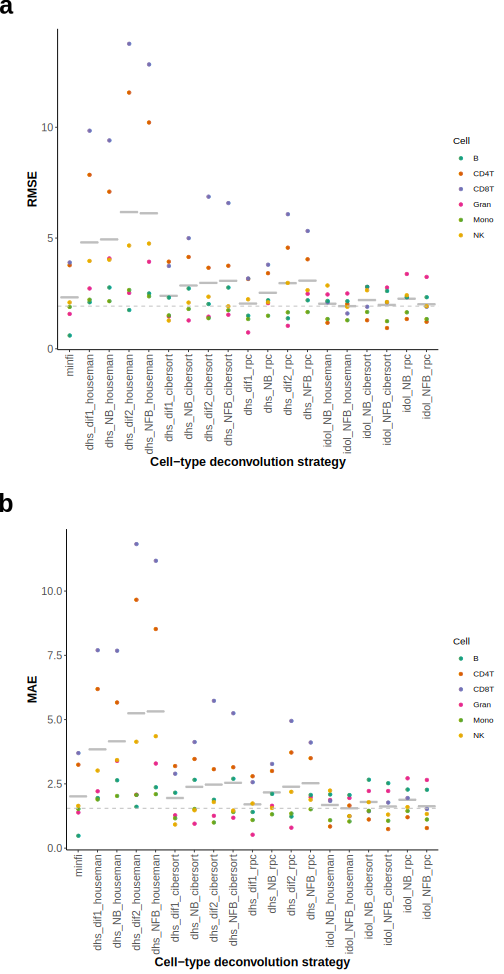
\includegraphics[width=0.7\textwidth]{C2_Fig4}
	\caption[Benchmarking of the cell-type deconvolution strategies in blood: $RMSE$ and $MAE$]{Benchmarking of the cell-type deconvolution strategies in blood. The x-axis shows the different strategies that were tested (for a detailed description see Fig.~\ref{fig:sc2_fig4}). The y-axis shows the results for \textbf{a.} the root mean squared error ($RMSE$) and \textbf{b.} the mean absolute error ($MAE$) when comparing the predictions with the real proportions of cells in a gold-standard dataset (GSE77797) \citep{Koestler2016}. The grey horizontal solid lines represent the mean for the $RMSE$ or the $MAE$ across cell types and the grey dashed line the minimum of these values.}
	\label{fig:c2_fig4}
\end{figure}

\begin{figure}[htbp!] 
	\centering    
	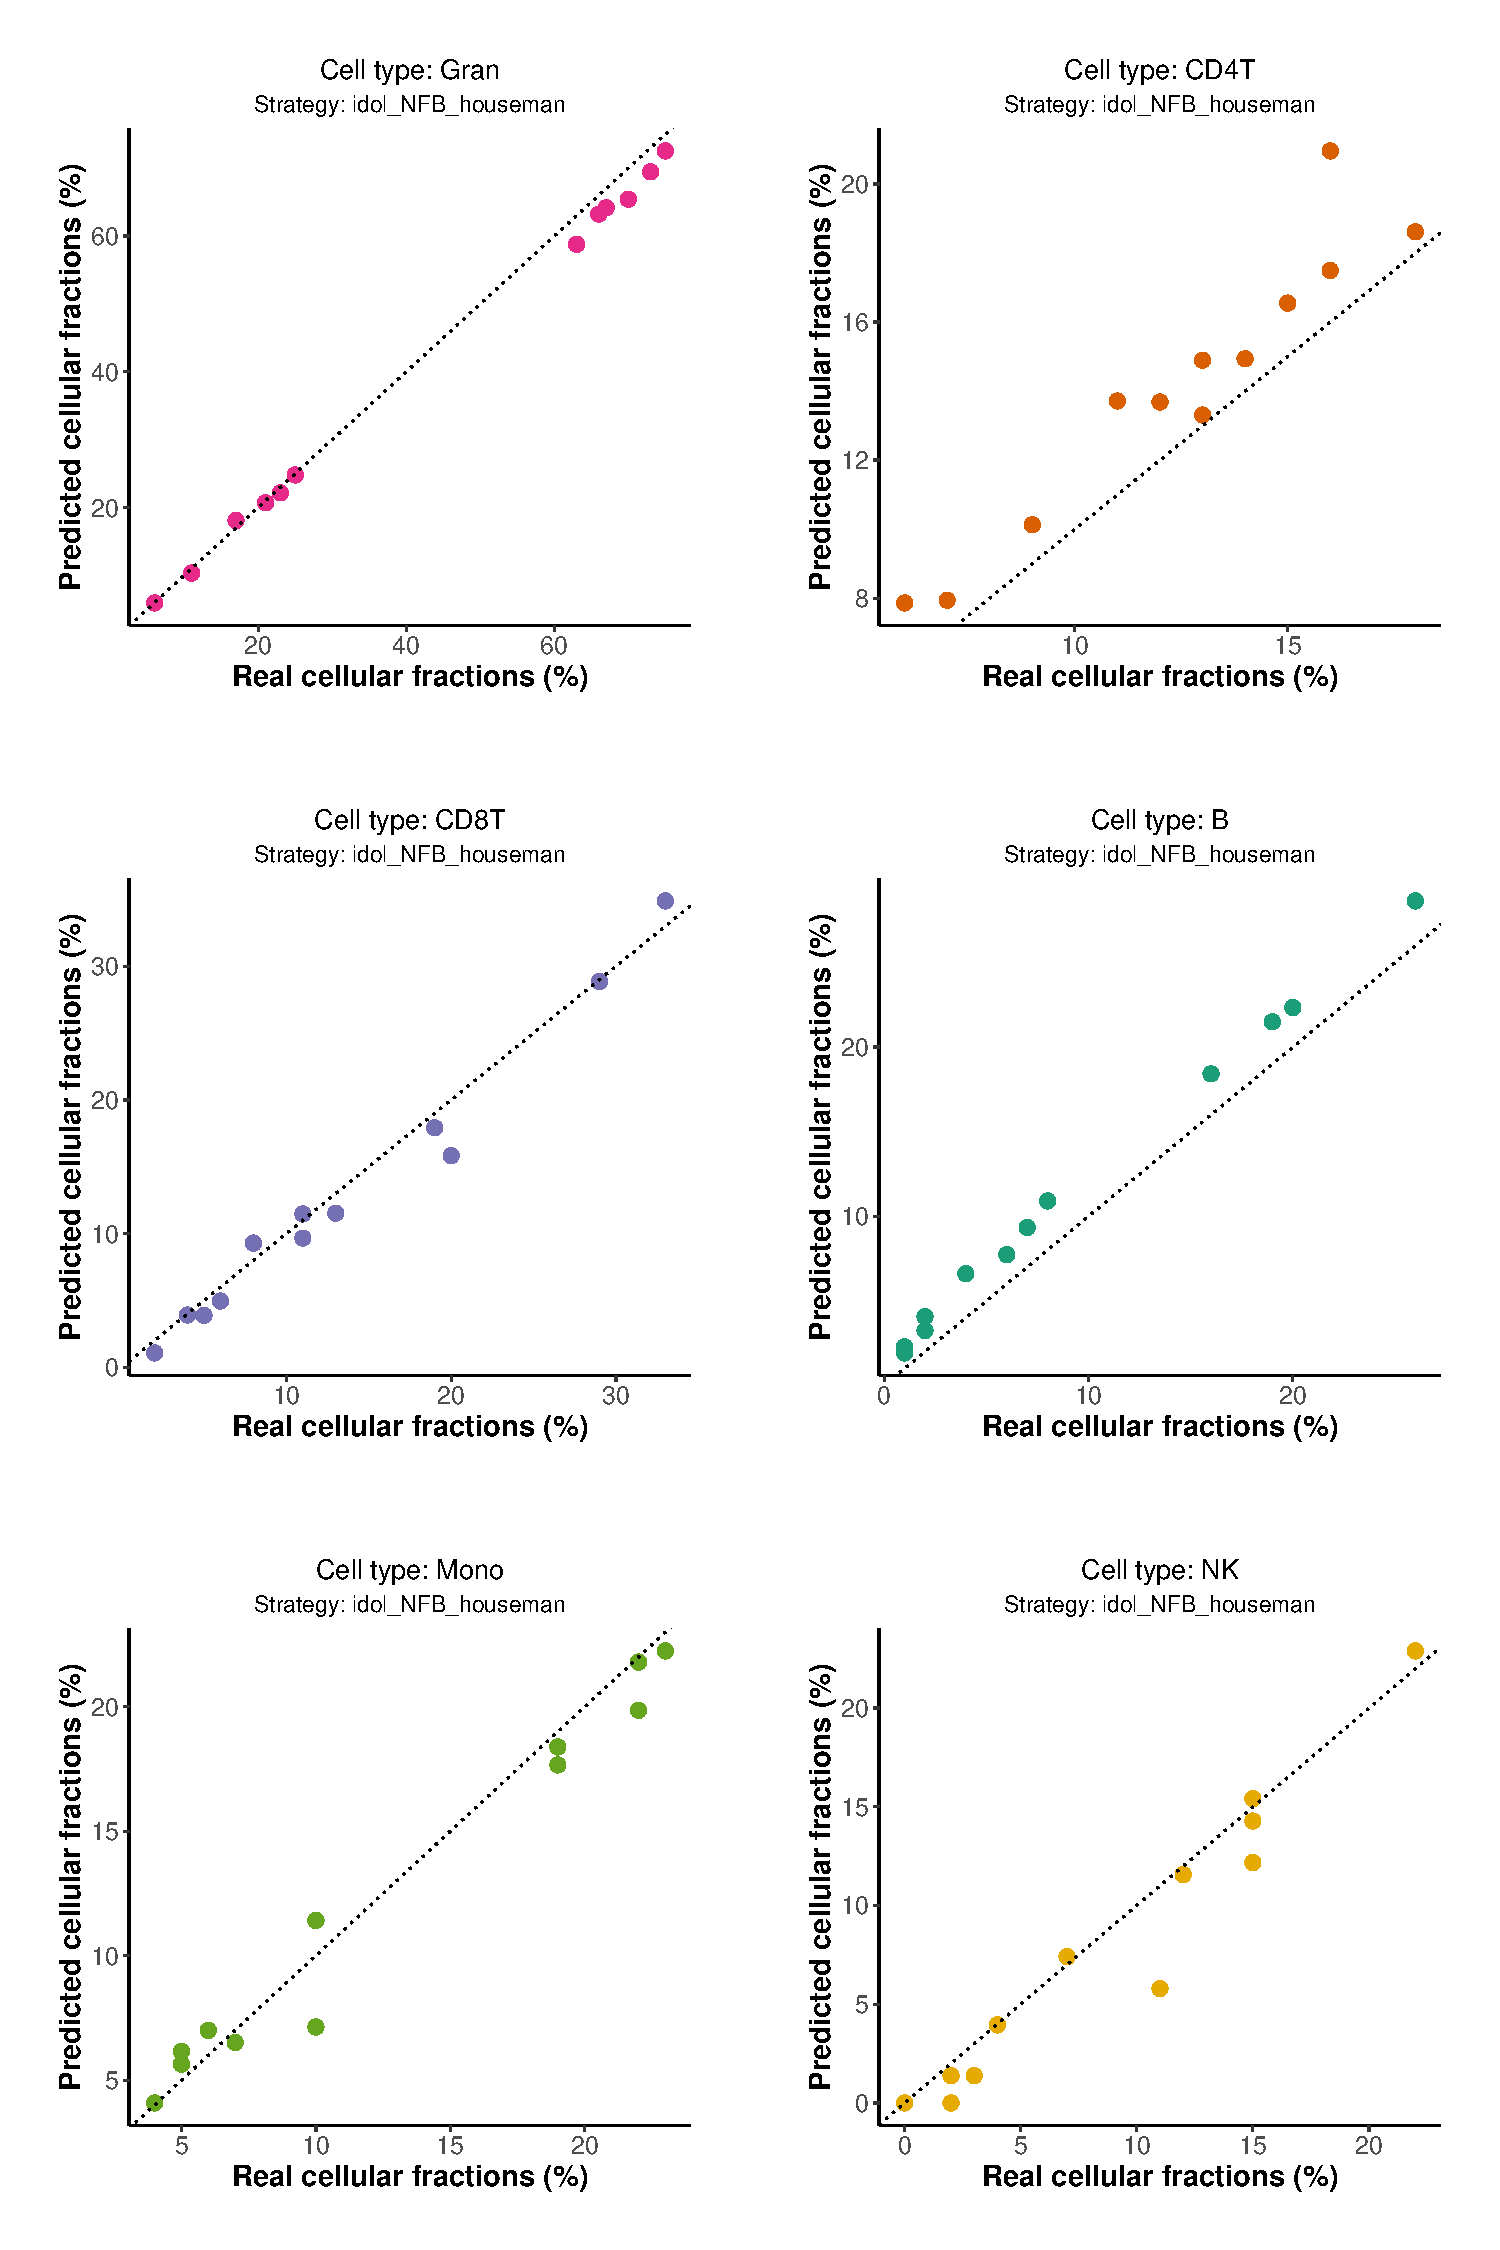
\includegraphics[width=0.9\textwidth]{C2_Fig5}
	\caption[Predictions obtained for each blood cell type using the optimal deconvolution strategy]{Comparison of the predictions for the different cell types using the optimal deconvolution strategy (`idol\_NFB\_houseman') with the real cell type fractions in the gold-standard dataset (GSE77797) \citep{Koestler2016}. Each point corresponds to a different sample in the gold-standard. The black dashed line represents the diagonal to aid visual interpretation.}
	\label{fig:c2_fig5}
\end{figure}


Next, I ran the optimal blood cell-type deconvolution strategy in the DNA methylation dataset that I built from healthy individuals (Table~\ref{table:c2_table1}). The main goal of this analysis was to provide blood cell type proportions that can be used as covariates as part of the epigenetic clock modelling (see section~\ref{s:2.2.2}). However, this also allowed me to broadly quantify the \textbf{changes in blood composition that occur during human ageing} (Fig.~\ref{fig:c2_fig6}). The mammalian immune system undergoes dramatic changes during ageing. These changes are normally referred as \textit{immunosenescence} and can be broadly defined as a decline in immune system functionality and its ability to fight infections, which results in an increase in morbidity and mortality with age \citep{Nikolich-Zugich2018}. Furthermore, human ageing is also characterised by an increase in chronic, low-grade inflammation referred as \textit{inflammageing}, which is thought to contribute to the development of age-related diseases (such as atherosclerosis, type 2 diabetes, Alzheimer’s disease and osteoporosis) \citep{Franceschi2007}.

\bigskip

In my dataset, I observe the following (Fig.~\ref{fig:c2_fig6}):

\begin{itemize}
	
	\item A relative decrease in cell types from the adaptive immune system (CD4$^+$ T cells, CD8$^+$ T cells and CD19$^+$ B cells). Interestingly, the decline in CD8$^+$ T cells was more pronounced (i.e. higher absolute value of the slope) than in the case of CD4$^+$ T cells, which has been previously reported \citep{Czesnikiewicz-Guzik2008}. 
	
	\item A relative increase in cell types from the innate immune system (granulocytes, CD14$^+$ monocytes and CD56$^+$ natural killer cells).
	
\end{itemize}

These results are highly consistent with the literature \citep{Jaffe2014,Czesnikiewicz-Guzik2008,Kuranda2011,Chen2016a,Seidler2010,Manser2016}, which validates the methodology for cell-type deconvolution that I have used. These variations in blood cell composition may be caused by the age-related changes that happen in the two primary lymphoid organs: the bone marrow (whose hematopoietic stem cells exhibit reduced self-renewal potential and increased skewing towards myelopoiesis) and the thymus (which undergoes tissue involution)  \citep{Chinn2012}. 

\bigskip

This analysis provides a preliminary overview of the blood cell composition landscape during human ageing. However, only relative changes in blood composition were quantified and the analysis is limited by the `cell types' that I have deconvoluted (e.g. granulocytes include different cell types, different subsets of monocytes exist, etc.), which means that these conclusions must be taken with care \citep{Nikolich-Zugich2018}. Furthermore, the sex of the individual can influence the proportions of blood leukocytes \citep{Chen2016a} and it should be taken into account in future analyses. 

\begin{figure}[htbp!] 
	\centering    
	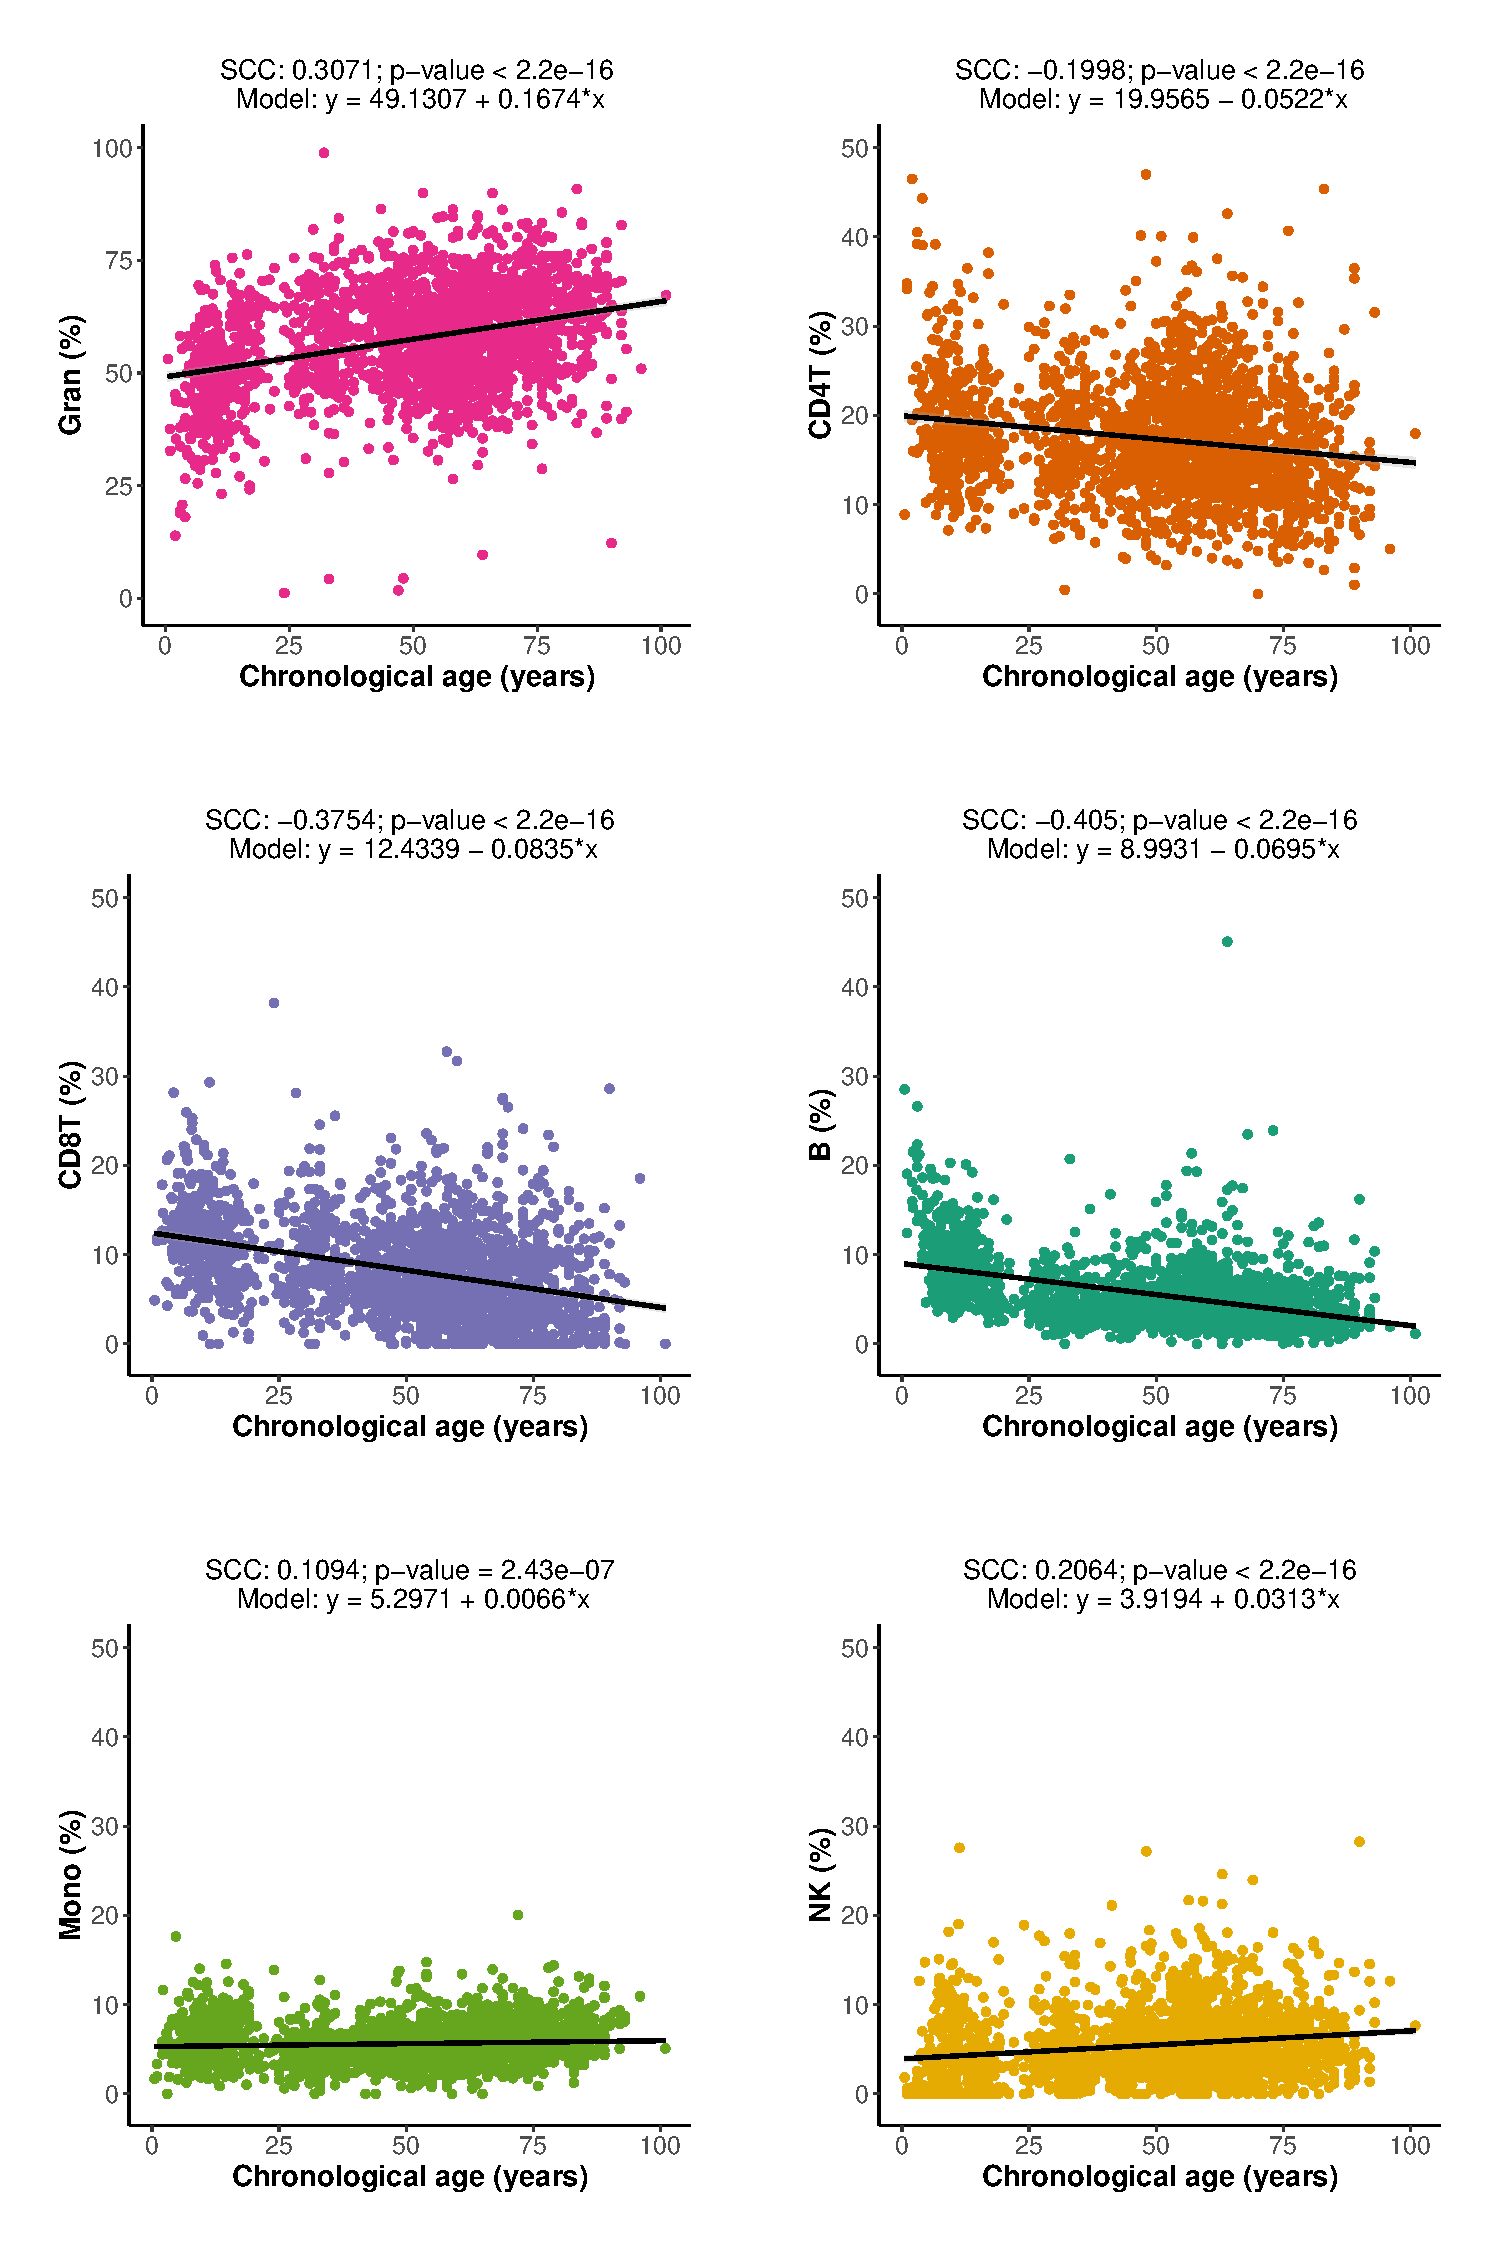
\includegraphics[width=0.9\textwidth]{C2_Fig6}
	\caption[Changes in blood cell composition during human ageing]{Changes in blood cell composition during human ageing. Scatterplots showing the changes in the proportions of the six cell types considered (inferred using the cell-type deconvolution strategy) as a function of chronological age. Each point represents a different DNA methylation human sample from Table~\ref{table:c2_table1}. The black line displays the linear model \%cell\_type $\sim$ Age (see section~\ref{s:2.4} for more details on linear modelling), with the slope and intercept shown in the titles. The Spearman's correlation coefficient (\acrshort{SCC}) and the p-value associated with it are also displayed.}
	\label{fig:c2_fig6}
\end{figure}



\smallskip

\subsection{Identifying differentially methylated positions during ageing} \label{s:2.1.4}

\smallskip

Differential methylation analysis is one of the most common types of downstream analyses in the context of DNA methylation data \citep{Wilhelm-Benartzi2013,Morris2015,Teschendorff2018}. It involves finding associations between the DNA methylation levels at specific CpG sites in the genome (a.k.a. differentially methylation positions or \acrshort{DMPs}) and a given phenotypic variable of interest (e.g. a specific disease, when compared with a healthy sample). It is worth mentioning that DMPs are also called differentially methylated cytosines (\acrshort{DMCs}) in the literature \citep{Teschendorff2018}.

\bigskip

In order to study the changes that the methylome undergoes during physiological ageing, it is useful to identify differentially methylated positions during ageing (\acrshort{aDMPs}) i.e. individual cytosines (normally found in a CpG context) that change their methylation status as a function of chronological age. Linear models, widely used in the context of differential RNA expression analysis \citep{Ritchie2015}, can also been adapted to find aDMPs \citep{Zhuang2012,Teschendorff2018}. In the case of a continuous variable (such as chronological age) the association is performed using a linear regression modelling framework \citep{Zhuang2012} (see section~\ref{s:2.4} for a short description of linear regression and the nomenclature used throughout this thesis). Briefly, for each probe in the methylation array, I fitted the following \textbf{linear regression models} to the data from the healthy individuals:

\begin{itemize}

	\item \textbf{A model with cell composition correction} (\acrshort{CCC}). As I have shown previously, the different blood cell types change their abundance with age. Therefore, in order to maximise the chances of finding aDMPs that are conserved across different cell types, it is important to include the estimated cell proportions as covariates in the model:
	
	\begin{align} \label{eq:2.10}
	Beta \sim Age + Sex+ Gran + CD4T + CD8T + B + Mono + NK + PC1 + ... + PC17
	\end{align}
	
	where $Beta$ is the $\beta$-value for the array probe being evaluated; $Age$ is the chronological age (in years) of the samples; $Sex$ encodes for the sex of the samples (0/1); $Gran$, $CD4T$, $CD8T$, $B$, $Mono$ and $NK$ are the cell type proportions from the samples as calculated with my cell-type deconvolution strategy and $PCN$ is the $N$th principal component that captures technical variance and accounts for potential batch effects (see section~\ref{s:2.2.3} for more details).    
	
	\item \textbf{A model without CCC}, which can be expressed as:
	
	\begin{align} \label{eq:2.11}
	Beta \sim Age + Sex+ PC1 + ... + PC17
	\end{align}
	
	This leads to the identification of aDMPs which will be more confounded with the proportions of the different cell types (i.e. the change in $\beta$-value with age could be entirely driven by a change in a specific cell type that is differentially methylated at that particular probe).
	
\end{itemize}

Furthermore, for each probe, I calculated a p-value, based on $t$-statistics \citep{Teschendorff2018}, to assess whether the putative linear association between the methylation status and chronological age was significant or not (at a significance level of $\alpha=0.01$ after applying Bonferroni correction to account for multiple testing, see section~\ref{s:2.4} for more details). I used a customised version of the \textit{dmpFinder} function in the \textit{minfi} R package \citep{Aryee2014} to identify the aDMPs, which internally uses the \textit{limma} framework \citep{Ritchie2015}. Given the big sample size ($N = 2218 \gg 10$), I did not use variance shrinkage (i.e. empirical Bayes moderated $t$-statistics) as part of the statistic calculations \citep{Ritchie2015}.  

\bigskip

An overview of the different aDMPs (with and without CCC) identified in the healthy individuals can be found in Figure~\ref{fig:c2_fig7}. \textbf{Around $30\%$ of the blood methylome (at least according to the 450K array) is affected by the ageing process} during human lifespan. However, it is worth mentioning that Bonferroni correction provides a very conservative picture of the methylomic changes (when compared with other methods to control for type-I error, like \acrshort{FDR}) and it is likely that an even greater proportion of the methylome is indeed altered with age \citep{Zhu2018}. CpG sites can become both hypomethylated (i.e. lose methylation with age) or hypermethylated (i.e. gain methylation with age). Importantly, the effect sizes of the age coefficient (i.e. the observed changes in the $\beta$-values per year) are generally small. More specifically, in the model with CCC, the median age coefficient for the hypomethylated aDMPs is -0.000426 (equivalent to a -4.26\% methylation change over 100 years of human life) and for hypermethylated aDMPs is 0.000437 (equivalent to a +4.37\% methylation change over 100 years of human life). This is consistent with the progressive functional decline observed during ageing \citep{Lopez-Otin2013}. It is worth mentioning that around $50\%$ of the CpG sites that constitute the Horvath epigenetic clock are blood aDMPs according to my analysis (Fig.~\ref{fig:c2_fig7}c,d). Overall, these results are consistent with previous studies \citep{Slieker2016,Slieker2018,Zhu2018,VanDongen2016}. 

\begin{figure}[htbp!] 
	\centering
	\vspace*{2mm}    
	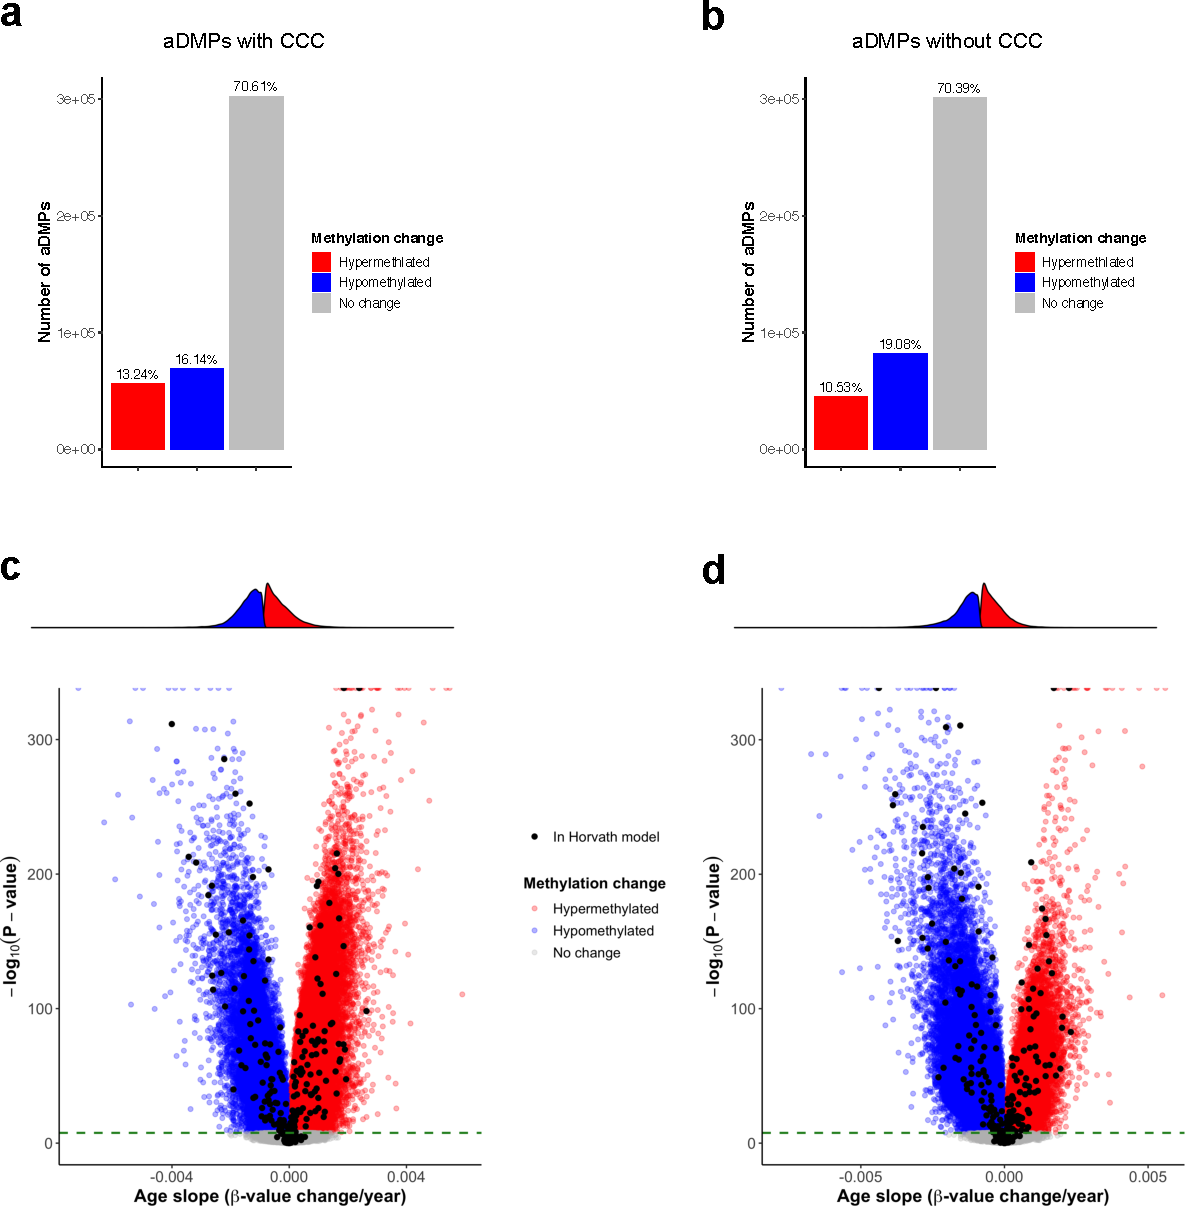
\includegraphics[width=1\textwidth]{C2_Fig7}
	\vspace*{2mm}
	\caption[Changes in the blood methylome during human ageing]{The blood methylome changes during physiological human ageing. \textbf{a.} Barplot showing the total number of differentially methylated positions during ageing (aDMPs) that were identified (in grey: probes that did not reach statistical significance). In this case, the model with cell composition correction (CCC) was applied. \textbf{b.} As in a., but using the model without CCC. \textbf{c.} Volcano plot showing the relationship between the p-value (y-axis) and the effect size (x-axis) of the age coefficient for each one of the array probes (each point represents a probe). Those probes above the dashed green line ($\alpha=0.01$ after Bonferroni correction) are the identified aDMPs. Above the volcano plot, a density plot captures the distributions of the age coefficient for the hypermethylated aDMPs (in red) and the hypomethylated aDMPs (in blue). In this case, the model with CCC was applied. The black points are the 353 CpG probes that constitute the Horvath epigenetic clock model \citep{Horvath2013}. \textbf{d.} As in c., but using the model without CCC.}
	\label{fig:c2_fig7}
\end{figure}

\bigskip

Next, I looked at the top 100 aDMPs that were identified (according to their p-value and $t$-statistic, Fig.~\ref{fig:sc2_fig6} and Fig.~\ref{fig:c2_fig8}). The first aDMP in the list was cg16867657, a probe that consistently gains methylation with age (Fig.~\ref{fig:c2_fig8}a) and has been previously identified as the strongest aDMP across tissues and human populations in several studies  \citep{Slieker2018,Hannum2013,Garagnani2012,Zbiec-Piekarska2015,Bacalini2017,Gopalan2017}. cg16867657 is associated with the CpG island in the promoter of the ELOVL2 gene, which encodes an enzyme that catalises one of the reactions in the elongation of polyunsaturated fatty acids \citep{Gopalan2017}. Furthermore, other aDMPs that were located among my top hits have previously been reported as well (such as cg06639320 in the FHL2 gene, which is the second aDMP, Fig.~\ref{fig:c2_fig8}b) \citep{Garagnani2012}. These results validate the statistical methods used so far to process the DNA methylation data and to identify aDMPs. 


\begin{figure}[htbp!] 
	\centering    
	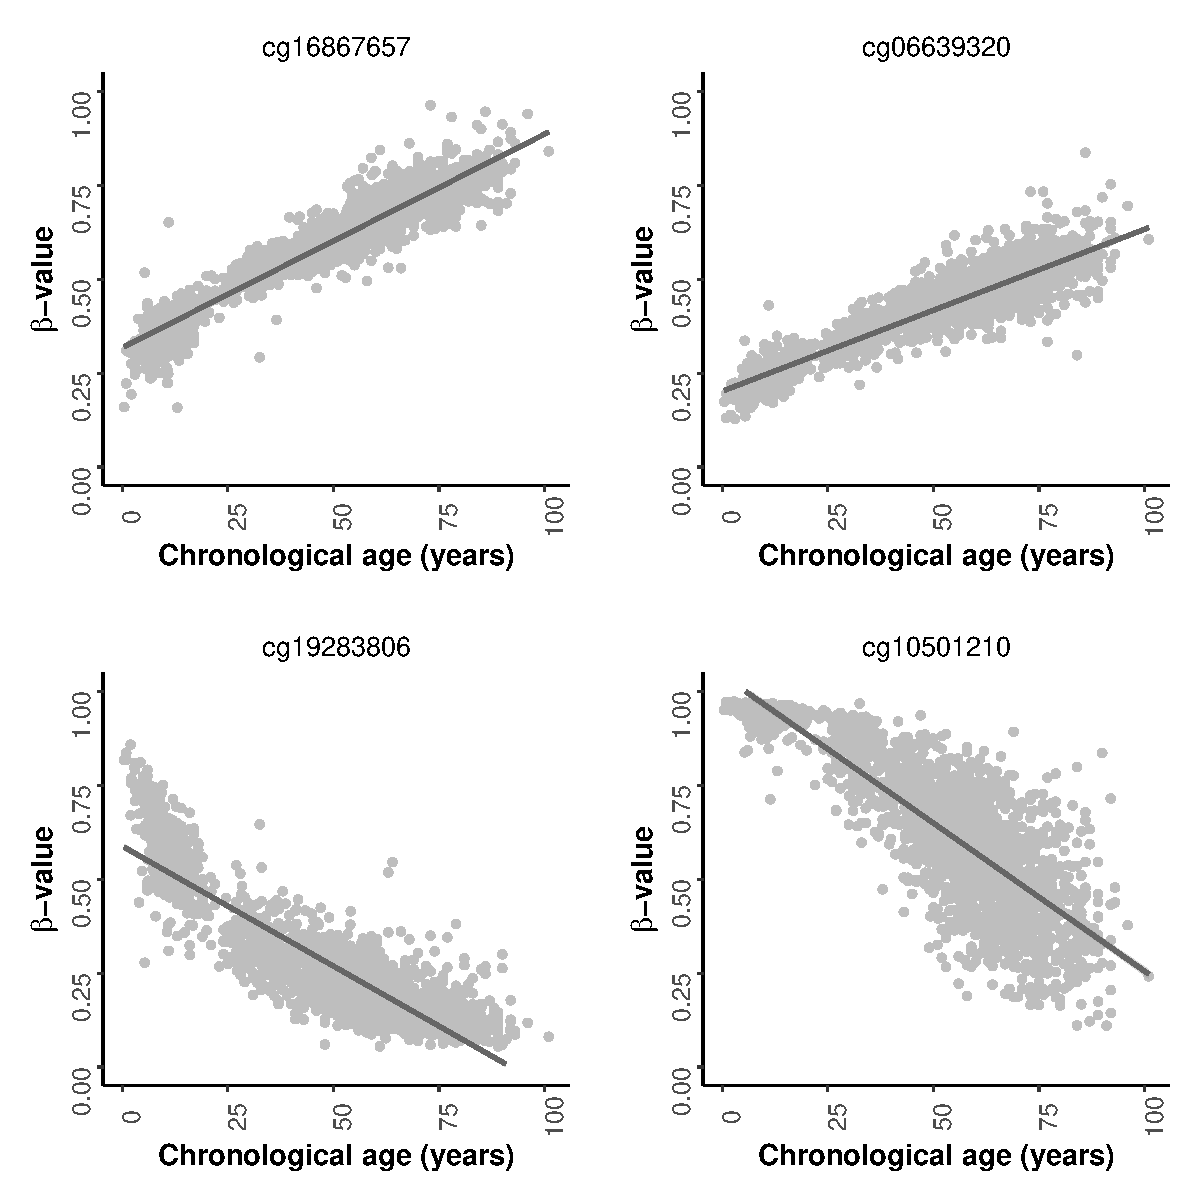
\includegraphics[width=0.9\textwidth]{C2_Fig8}
	\caption[Changes in the $\beta$-values of four different aDMPs]{Changes in the $\beta$-values of four differentially methylated positions during ageing (aDMPs) in the blood of the healthy individuals. cg16867657 and cg06639320 are the top aDMPs that gain methylation with age (i.e. become hypermethylated) according to the model that accounts for cell composition correction (CCC). cg19283806 and cg10501210 are the top aDMPs that lose methylation with age (i.e. become hypomethylated) according to the model that accounts for CCC. In order to aid visualisation, the black line displays the linear model $\beta$-value $\sim$ Age.}
	\label{fig:c2_fig8}
\end{figure}

\bigskip

It is important to mention that not all the CpG sites change their DNA methylation levels with age in a perfectly linear manner. For instance, the two top hypomethylated aDMPs (Fig.~\ref{fig:c2_fig8}c,d) modify their rate at ages 20-25 years. This was already recognised by Horvath \citep{Horvath2013} and that is why he transformed the age into a logarithmic scale before the age of 20 years in order to improve the model fit (see section~\ref{s:2.2.1}). Furthermore, genetic background can have a significant effect on the DNA methylation patterns and interact with the ageing process to shape the epigenome \citep{Hannum2013,VanDongen2016}. Unfortunately, I did not have genetic data for the healthy individuals but this could help to refine the identification of aDMPs in the future. Additionally, it would be interesting to apply methods to control for bias and inflation in the test statistic, by estimating the empirical null distribution of the observed set of test statistics \citep{VanIterson2017}. Finally, other types of epigenetic features can be derived to understand the effects of ageing in the epigenome, such as variably methylated positions during ageing (\acrshort{aVMPs}) \citep{Slieker2016}, differentially methylated regions (\acrshort{DMRs}, which consider several correlated CpGs at the same time) \citep{Teschendorff2018} or differentially methylated cytosines in individual cell types (\acrshort{DMCTs}, which consider interactions between the phenotypic variable and the proportions of cell types) \citep{Zheng2018}.


\smallskip

\subsection{Shannon methylation entropy} \label{s:2.1.5}

\smallskip

Shannon entropy ($H$) can be used in the context of DNA methylation analysis to \textbf{estimate the information content stored in a given set of CpG sites} \citep{Wang2017,Slieker2016,Hannum2013,Xie2011,Jenkinson2017}. I calculated it using the same approach as in \citet{Hannum2013}:

\begin{align}
H = - \frac{1}{N} \cdot \sum_{i=1}^{N}[\beta_i \cdot \log_2(\beta_i) + (1-\beta_i) \cdot \log_2(1-\beta_i)]
\end{align}

where $\beta_i$ represents the methylation $\beta$-value for the $i$th array probe (or CpG site) and $N=428266$ if all the array probes that passed the pre-processing pipeline are considered (i.e. genome-wide, ot at least array-wide). Shannon entropy is minimised when the methylation levels of all the CpGs are either 0\% or 100\%, and maximised when all of them are 50\% (Fig.~\ref{fig:c2_fig9}).

\bigskip

Next, I calculated the genome-wide  Shannon entropy for the blood samples in the healthy individuals. Consistent with previous reports \citep{Slieker2016,Hannum2013,Wang2017,Jenkinson2017},  \textbf{the genome-wide Shannon entropy associated with the methylome increases during ageing} (Fig.~\ref{fig:c2_fig10}a; Spearman correlation coefficient $= 0.1985$; p-value $= 3.8281 \cdot 10^{-21}$), which implies that the epigenome loses information content. Finally, it is worth mentioning that I observed a remarkable batch effect on the Shannon entropy calculations, which can generate high entropy variability for a given age (Fig.~\ref{fig:c2_fig10}b). However, after removing potential outlier batches (such as GSE41273, GSE59065 or GSE97362) the increase of Shannon methylation entropy during ageing was still consistent. Thus, accounting for technical variation (see section~\ref{s:2.2.3}) becomes crucial when assessing this type of data, even after careful pre-processing. 

\begin{figure}[htbp!] 
	\centering
	\vspace*{3mm}    
	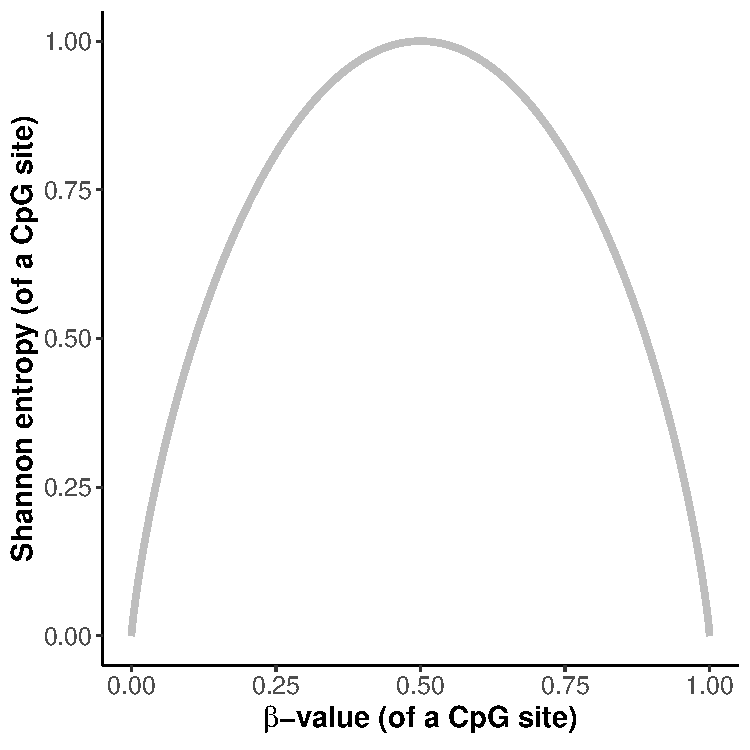
\includegraphics[width=0.5\textwidth]{C2_Fig9}
	\caption[Relationship between the $\beta$-value and the Shannon entropy at a given CpG site]{Plot showing the relationship between the $\beta$-value and the methylation Shannon entropy at a given CpG site (in my case, at a given array probe).}
	\label{fig:c2_fig9}
\end{figure}

\begin{figure}[htbp!] 
	\centering
	\vspace*{2mm}    
	\includegraphics[width=1\textwidth]{C2_Fig10}
	\caption[Genome-wide methylation Shannon entropy during physiological ageing]{\textbf{a.} Scatterplot showing the changes in genome-wide methylation Shannon entropy during ageing in the healthy individuals. Each sample is represented by one point. The black line displays the linear model Entropy $\sim$ Age. \textbf{b.} Same as in a., but colouring the samples according to the batch where they came from.}
	\label{fig:c2_fig10}
\end{figure}


\smallskip

\section{Behaviour of Horvath's epigenetic clock during ageing}

\smallskip

\subsection{Calculating epigenetic age using Horvath's epigenetic clock} \label{s:2.2.1}

\smallskip

Steve Horvath's model, originally published in 2013 \citep{Horvath2013}, is without any doubt the most widely used epigenetic clock in the literature. Given that it works across tissues with high accuracy and that it has been validated in many human cohorts, I have used it as the main tool to quantify epigenetic ageing in this work. 

\bigskip

Horvath's model measures epigenetic age (a.k.a. \textit{DNAmAge}) by making use of the DNA methylation levels at 353 CpG sites, as quantified with the Illumina methylation arrays (27K or 450K). Previous studies have generally employed a ready-to-use online calculator for \textit{DNAmAge} provided by Steve Horvath \citep{Horvath2013b}. This has clearly simplified the computational process and helped a lot of research groups to test the behaviour of the epigenetic clock in their system of interest. However, this has also led to the treatment of the epigenetic clock as a `black-box’, without critical assessment of the statistical methodology behind it. Therefore, I decided to replicate the original code and to make it available in a GitHub repository for the scientific community to be used \citep{Martin-Herranz2019}. Furthermore, I tested the impact of different steps involved in the estimation of epigenetic age acceleration (EAA), including the presence/absence of background correction, removal of technical variation from batch effects and the importance of the age distribution when fitting the control models, which I discuss in the following sections. 

\bigskip

The main pipeline to calculate the epigenetic age (\textit{DNAmAge}) from a sample has the following steps (some of them are shared with the previously described pipeline for DNA methylation pre-processing in section~\ref{s:2.1.2}):

\begin{enumerate}
	
	\item \textbf{Background correction}. I implemented a pipeline that starts with the raw DNA methylation data (IDAT files) for a sample. First, I tested the effect of applying \textit{noob} background correction, before calculating the $\beta$-values, on the median absolute error (MAE) of the predictions (see section~\ref{s:2.2.2}).  Background correction did not have a major impact in the final predictions as long as I also corrected for batch effects (Fig.~\ref{fig:sc2_fig7}, Fig.~\ref{fig:c2_fig13}c, see section~\ref{s:2.2.3}). Therefore, I decided to keep the \textit{noob} background correction for consistency with the other pre-processing pipeline.
	
	\item \textbf{Quality control}. I applied the same criteria as previously described in section \ref{s:2.1.2}.
	
	\item \textbf{Probe filtering}. Horvath's model was originally trained starting with 21368 array probes that had the following characteristics \citep{Horvath2013}:
	
	\begin{itemize}
		
		\item They were shared between the 27K and 450K methylation arrays.
		
		\item They had $\leq$ 10 missing values across all the training data.
		
	\end{itemize}
	
	 Therefore, these were the probes selected for downstream analysis.
	
	\item \textbf{$\beta$-value calculation}. $\beta$-values were calculated as previously described in section \ref{s:2.1.2}. It is worth mentioning that Horvath's original code includes two alternatives for the imputation of missing $\beta$-values:
	
	\begin{itemize}
		
		\item Slow imputation (applied when the number of missing $\beta$-values is < 3000). In this case, $k$-nearest neighbours (\acrshort{KNN}) is used. KNN imputation borrows information from the DNA methylation profiles of the most similar probes (the neighbours) according to a metric (normally the Euclidean distance). The \textit{impute.knn} function from the \textit{impute} R package can be used for these purposes \citep{Troyanskaya2001}.
		
		\item Fast imputation (applied when the number of missing $\beta$-values is $\geq$ 3000). In this case, the values from the blood gold-standard (see below) can be used as the imputed values.
		
	\end{itemize}
	
	In the case of my dataset, no missing values were present for the $21368$ probes so there was no need to perform imputation.
	
	\item \textbf{Gold-standard normalisation}. A modified version of BMIQ normalisation is used \citep{Teschendorff2012}. In this case, instead of mapping the distribution of the Infinium II probes to the distribution of Infinium I probes, the mapping is done from the distribution of the 21368 probes in the sample to the distribution of a previously derived gold-standard for the same set of probes. This gold-standard was created by taking the average $\beta$-values for the 21368 probes across all the whole blood samples from \citep{Horvath2012}.
	
	\item \textbf{Calculating epigenetic age} (\textit{DNAmAge}). As previously observed for some of the aDMPs, the rate of $\beta$-value change can be different before and after adult age (Fig.~\ref{fig:c2_fig8}). For this reason, Horvath performed a transformation of the chronological age before training the model:
	
	\begin{align}
	f(c) = c_t =  
	\begin{cases}
	\ln\left(\frac{c+1}{a+1}\right) &\text{if: } c\leq a \\
	\left(\frac{c-a}{a+1}\right) &\text{if: } c>a \\
	\end{cases}
	\end{align} 
	
	where $c_t$ is the transformed chronological age that was used as the dependent variable during training, $c$ is the chronological age (in years) and $a$ is the adult age (for humans, 20 years). This transformation allows accounting for a relationship between chronological age and methylation changes that is logarithmic until adult age and linear afterwards (Fig.~\ref{fig:c2_fig11}). 
	
	\begin{figure}[htbp!] 
		\centering
		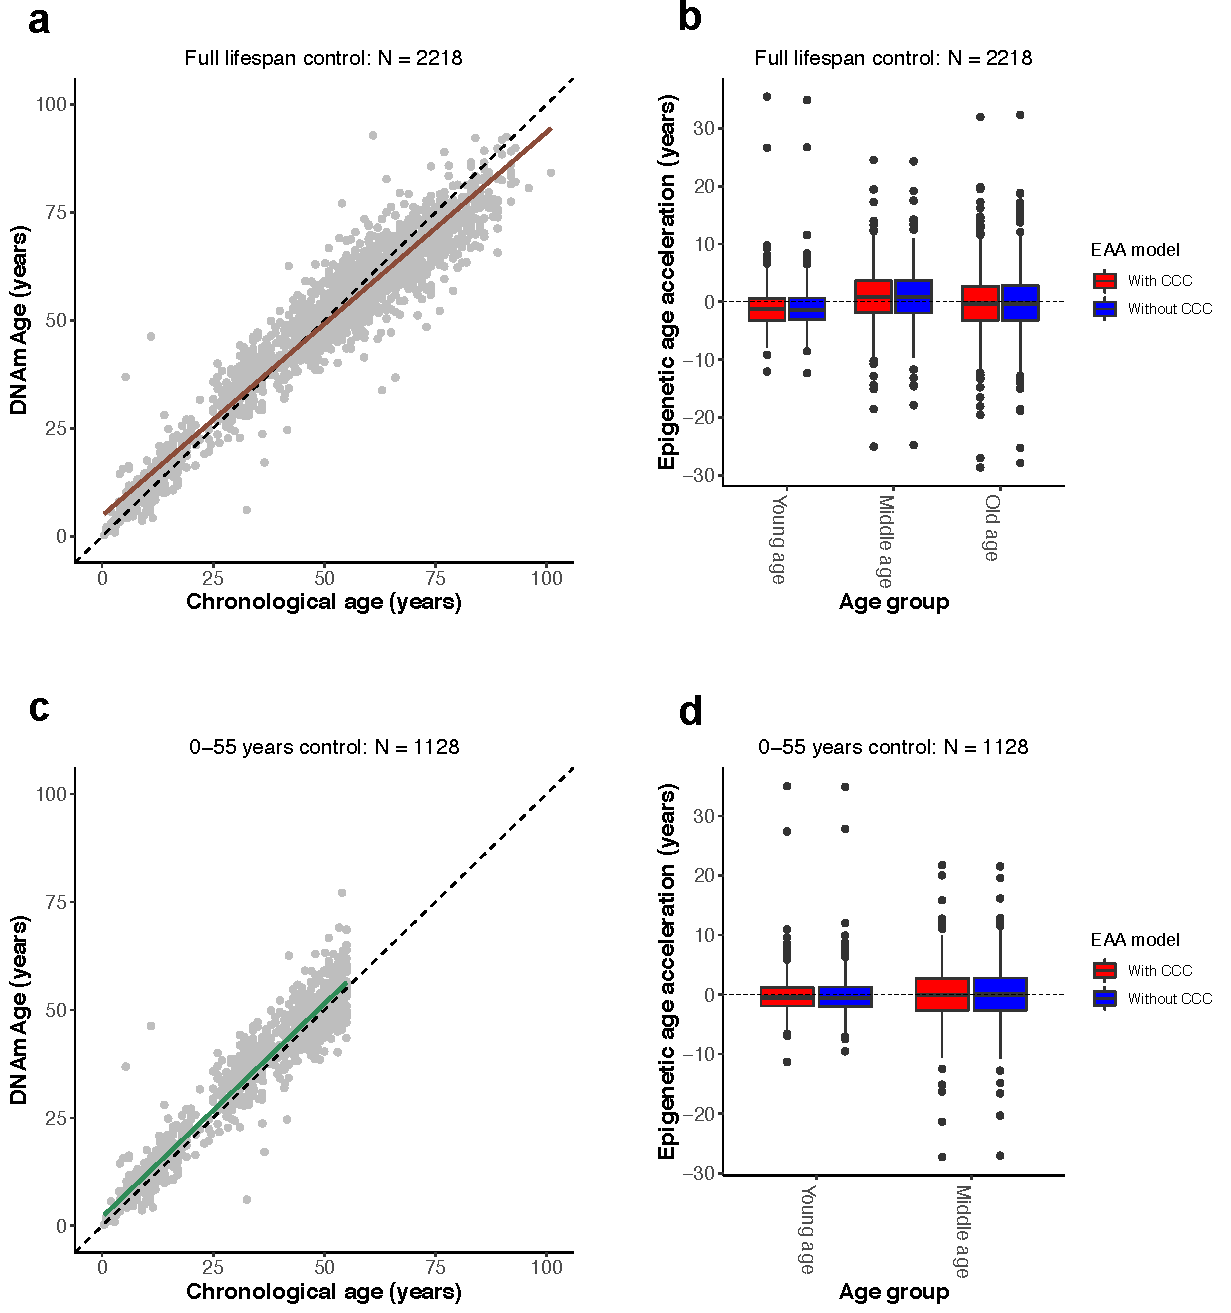
\includegraphics[width=0.5\textwidth]{C2_Fig11}
		\vspace*{2mm}    
		\caption[Transforming chronological age in Horvath's model]{Plot showing the relationship between the chronological age in years ($c$) and the transformed chronological age ($c_t$) in Horvath's model. This transformation allows accounting for different rates of $\beta$-value change before and after adult age (20 years in humans, as pointed out by the dashed black line).}
		\label{fig:c2_fig11}
	\end{figure} 
	
	Given a sample to predict, the epigenetic age can then be calculated as:
	
	\begin{align}
	DNAmAge = g(\hat{c}_t) = g(\hat{\beta}_0 + \sum_{i=1}^{353}\hat{\beta}_i \cdot x_i)
	\end{align}
	
	where $\hat{c}_t$ is the predicted transformed age according to Horvath's model, $\hat{\beta}_0$ is the intercept in the Horvath's model, $\hat{\beta}_i$ is the coefficient (weight) for the $i$th probe (only 353 probes are finally used), $x_i$ is the $\beta$-value for the $i$th probe after gold-standard normalisation and $g(\cdot)$ is the inverse of $f(\cdot)$, such that:
	
	\begin{align}
	g(\hat{c}_t) = f^{-1}(\hat{c}_t) = \hat{c} = 
	\begin{cases}
	e^{\hat{c}_t} \cdot (a+1) - 1 &\text{if: } \hat{c}_t \leq 0 \\
	\hat{c}_t \cdot (a+1) + a &\text{if: } \hat{c}_t > 0 \\
	\end{cases}
	\end{align} 
	
	where $\hat{c}$ is the predicted age according to Horvath's model (i.e. \textit{DNAmAge}).
	
\end{enumerate}


\smallskip


\subsection{Horvath's epigenetic clock measures physiological ageing} \label{s:2.2.2}

\smallskip

Using the methodology from the previous section, I calculated the epigenetic age (\textit{\acrshort{DNAmAge}}) in the blood of the healthy individuals. Given that these individuals are supposed to be disease-free, Horvath's epigenetic clock should predict epigenetic ages that are similar to the chronological age of the samples, and this was indeed the case (Fig.~\ref{fig:c2_fig12}a, Pearson's correlation coefficient (\acrshort{PCC}) $= 0.9671$, p-value $\approx 0$). This validates that Horvath's epigenetic clock does indeed measure the ageing process (at least in a cross-sectional population) and sets a foundation for the rest of the analyses presented in this thesis.

\bigskip

As mentioned in Chapter~\ref{c:1}, the difference between epigenetic age and chronological age is known as \textbf{epigenetic age acceleration} (\acrshort{EAA}), with a positive EAA (i.e. $DNAmAge > Age$) associated with several age-related health problems. In order to calculate the EAA for the healthy individuals, I fitted the following linear regression models (hereinafter referred as the \textit{control models}):

\begin{itemize}
	
	\item \textbf{With cell composition correction} (CCC):
	
	\begin{align} \label{eq:2.16}
	 DNAmAge \sim Age + Sex+ Gran + CD4T + CD8T + B + Mono + NK + PC1 + ... + PC17
	\end{align}
	
	where $DNAmAge$ is the epigenetic age calculated with Horvath's epigenetic clock; $Age$ is the chronological age (in years) of the samples; $Sex$ encodes for the sex of the samples (0/1); $Gran$, $CD4T$, $CD8T$, $B$, $Mono$ and $NK$ are the cell type proportions from the samples as calculated with my cell-type deconvolution strategy and $PCN$ is the $N$th principal component that captures technical variance and accounts for potential batch effects (see section~\ref{s:2.2.3} for more details). 
	
	Horvath's epigenetic clock was trained using multiple tissues and its predictions should be robust to changes in blood cell composition. However, previous studies have highlighted that adding this correction can improve the ability to detect `pure' ageing effects \citep{Chen2016,Horvath2016} (i.e. epigenetic age acceleration mainly caused by DNA methylation changes that happen in the nucleus of all cell types). For a given sample, the EAA$_{\text{with CCC}}$ is the residual from the model i.e. the difference between the actual $DNAmAge$ and the prediction from the control model (which is conceptually similar to the difference between $DNAmAge$ and chronological age, but accounting for the rest of covariates as well). The EAA$_{\text{with CCC}}$ that I have defined is very similar to the previously reported measure of `intrinsic EAA' (\acrshort{IEAA}) \citep{Chen2016,Horvath2016}.
	
	\item \textbf{Without CCC}:
	
	\begin{align} \label{eq:2.17}
	DNAmAge \sim Age + Sex+ PC1 + ... + PC17
	\end{align}
	
	In this case the residuals of the model are referred as the EAA$_{\text{without CCC}}$ for the different samples.
	
\end{itemize}

It is possible to calculate the overall accuracy of the predictions using the median absolute error ($MAE)$, that is calculated as:

\begin{align}
 	MAE = \mathrm{median}\left\{|EAA_i|\right\}
\end{align}

where $EAA_i$ is the epigenetic age acceleration for the $i$th sample calculated with one of the models (with CCC or without CCC). The $MAE$ for all the healthy individuals (full lifespan) in the control models should approach zero, and this was indeed what I observed ($MAE_{\text{with CCC}} = 2.7117$ years, $MAE_{\text{without CCC}} = 2.8211$ years). These results are below the original MAE reported by Horvath in his test set (3.6 years) \citep{Horvath2013}. However, it is worth mentioning that some of the samples from my healthy individuals (such as samples from batches GSE40279 and GSE42861) could have been used by Horvath as part of his training set \citep{Horvath2013}, and therefore these results must be interpreted carefully. 

\begin{figure}[htbp!] 
	\centering
	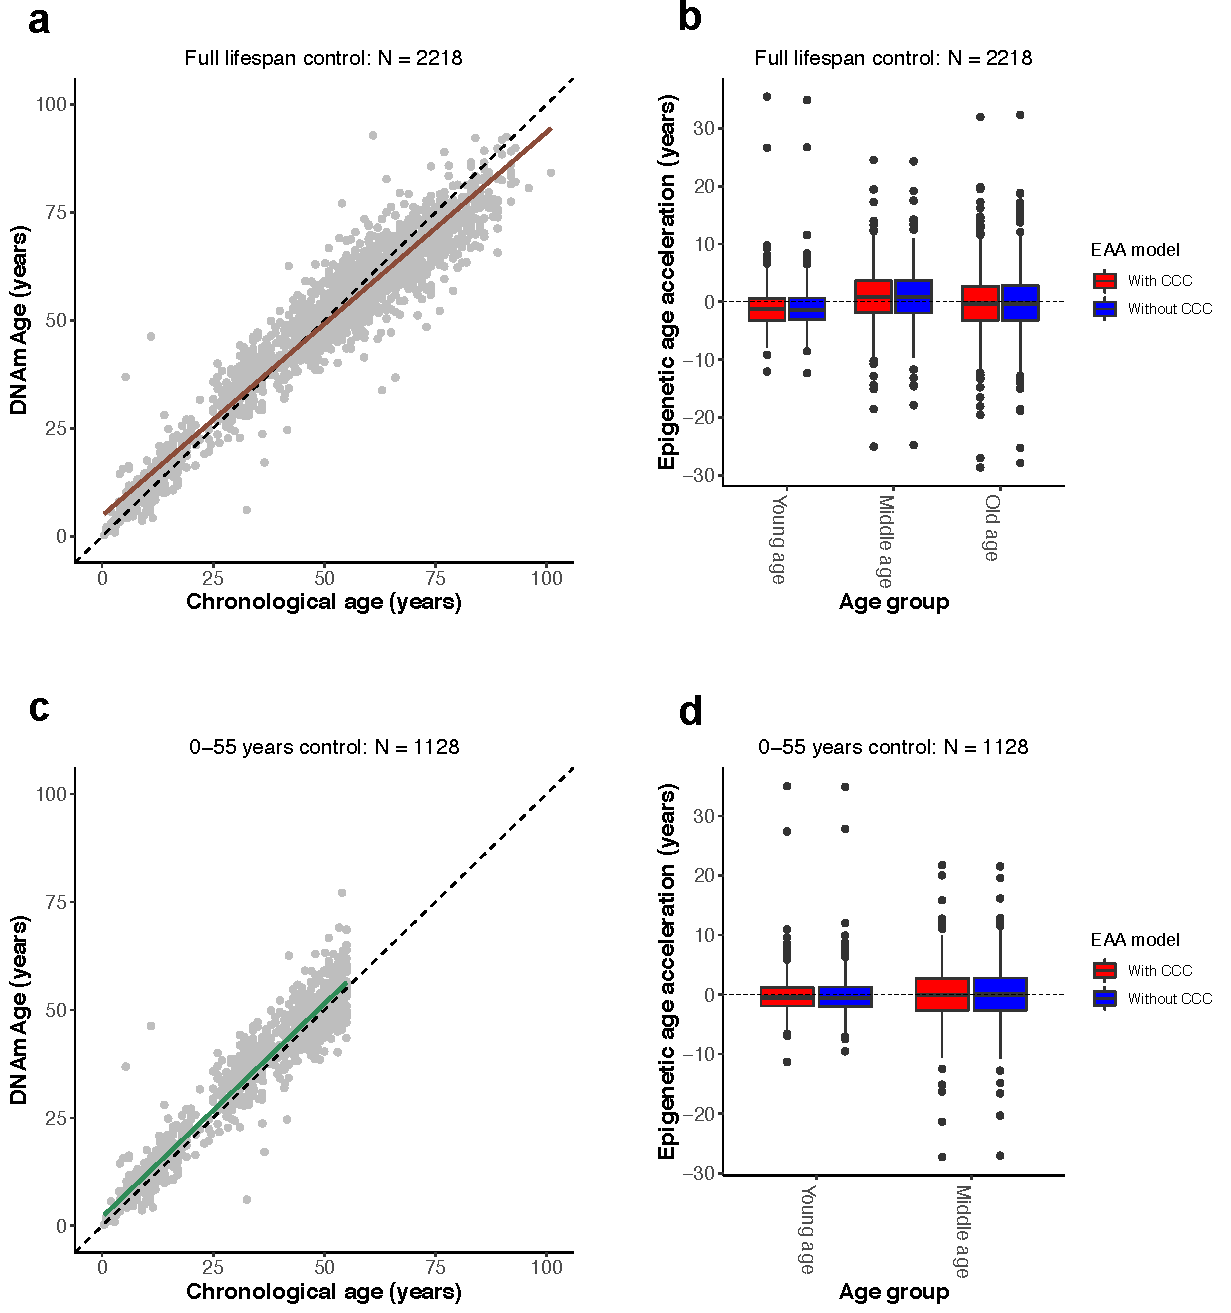
\includegraphics[width=1\textwidth]{C2_Fig12}
	\vspace*{2mm}    
	\caption[Horvath's epigenetic clock measures physiological ageing]{Horvath's epigenetic clock measures physiological ageing. \textbf{a.} Scatterplot showing the relationship between epigenetic age ($DNAmAge$) according to Horvath’s model \citep{Horvath2013} and chronological age of the samples for the healthy individuals. Each sample is represented by one point. The black dashed line represents the diagonal to aid visualisation. The solid brown line represents the linear model DNAmAge $\sim$ Age, which deviates from the diagonal if the full lifespan samples are used. \textbf{b.} Boxplots displaying the epigenetic age acceleration (EAA) distributions for different age ranges (young age: $\leq 20$ years; middle age: $20 < Age \leq 55$ years; old age: $> 55$ years) after fitting the control models to the full lifespan samples. The dashed black line represents $EAA = 0$, where the distributions should be centred around. This is not the case for the samples in the young age and middle age groups. In red: EAA model with cell composition correction (CCC). In blue: EAA model without CCC. \textbf{c.} As in a., but removing the samples in the old age group (> 55 years). The solid green line represents the linear model DNAmAge $\sim$ Age, which is much more similar to the diagonal if only young and middle age samples are considered. \textbf{d.} As in b., but fitting the control models to the samples in the young and middle age groups (0-55 years). The bias in the EAA is corrected in this case (the distributions are centred around zero for the different age groups).}
	\label{fig:c2_fig12}
\end{figure}   

\bigskip

Even though Horvath's model seems to predict epigenetic age accurately, it is also clear that some samples deviate substantially from the expected prediction. This is specially obvious for the older samples (> 55 years), that have a systematically younger epigenetic age than expected (see deviations from the diagonal in  Fig.~\ref{fig:c2_fig12}a). If a control model is fit to the full lifespan dataset (which contains around 50\% samples which are > 55 years), this leads to a model with a smaller than expected age coefficient (slope), which introduces a bias when estimating epigenetic age acceleration for different age groups (Fig.~\ref{fig:c2_fig12}b). Although many studies do not take this problem into account, this phenomenon has been previously reported in the context of humans \citep{ElKhoury2018,Marioni2018} and mice \citep{Stubbs2017}. However, to this date, it is unclear whether it represents a technical artefact or has a biological explanation (e.g. survivor bias of the older individuals, the molecular processes that drive ageing slow down with age, etc.). 

\bigskip

This highlights the importance of \textbf{having a properly age-matched control when performing analyses with the Horvath's epigenetic clock}. As expected, removing the older samples (> 55 years) from the control models corrected for this bias (Fig.~\ref{fig:c2_fig12}c,d) and reduced the $MAE$ ($MAE_{\text{with CCC}} = 2.2742$ years, $MAE_{\text{without CCC}} = 2.3237$ years). This is the strategy that I used when screening for epigenetic age acceleration in the context of developmental disorders (see Chapter~\ref{c:3}).

\smallskip

\subsection{Correcting for batch effects in the context of the epigenetic clock} \label{s:2.2.3}

\smallskip

As mentioned in the previous section, it is expected that, after fitting the control models, the EAA distributions of the samples from the healthy individuals should be centred around zero. However, when the principal components (\acrshort{PC}s) that capture technical variation were not included in the control models (see equations \ref{eq:2.16} and \ref{eq:2.17}), this was not the case for several batches (Fig.~\ref{fig:c2_fig13}a, Fig.~\ref{fig:sc2_fig8}a). Therefore, I hypothesised that technical variation can affect the predictions from Horvath's epigenetic clock and that batch effects need to be explicitly accounted for in this context, even after applying the internal normalisation step against the blood gold-standard \citep{Horvath2013}. This section explains how I implemented this batch effect correction (i.e. how I derived the principal components that capture technical variance across batches).

\bigskip

A batch effect is a systematic technical source of variation that is unrelated to the biological or scientific variables in a study \citep{Leek2010}. They affect low- and high-throughput measurements and can be caused by a wide variety of situations: different technicians performing the experiments, different laboratories generating the data, different lots of reagents or arrays used, etc. \citep{Leek2010}. Correcting for batch effects is crucial, especially when integrating data from different studies and sources \citep{Maksimovic2015}, as it is the case in the analyses presented in this thesis. Data generated by DNA methylation arrays is also affected by batch effects and several methods have been described in the literature to correct for them, normally at the level of probe intensities \citep{Fortin2014} or M-values \citep{Maksimovic2015,Price2018}. In the context of the epigenetic clock, previous attempts to account for technical variation have used the first five \acrshort{PC}s estimated directly from the DNA methylation data (presumably the $\beta$-values) \citep{Horvath2016a}. However, this approach potentially removes meaningful biological variation, especially in studies with global changes in DNA methylation, such as cancer \citep{Fortin2014} or developmental disorders (see Chapter~\ref{c:3}). Furthermore, given that Horvath's epigenetic clock was trained with data pre-processed using different strategies, it is unclear how applying an additional batch effect correction step to the intensities or $\beta$-values would impact the predictions \citep{Horvath2013a}.

\bigskip

Thus, I decided to correct for the potential batch effects when fitting the control models (see equations \ref{eq:2.16} and \ref{eq:2.17}). I make use of the \textbf{control probes present on the 450K array}, which have been shown to carry information about unwanted variation from a technical source (i.e. technical variance)  \citep{Maksimovic2015,Fortin2014,Gagnon-Bartsch2012}. These probes are designed to capture technical variance in negative controls, measure between-array differences and quantify the performance of different steps of the array protocol, such as bisulfite conversion, staining or hybridisation \citep{Fortin2014,Illumina2010}. I performed principal component analysis (PCA, with centering but not scaling using the \textit{prcomp} function in R) on the raw intensities of the control probes (847 probes $\cdot$ 2 channels $= 1694$ intensity values) for all the healthy individuals ($N=2218$) and the samples with developmental disorders (cases, $N=666$, see Chapter~\ref{c:3}). This showed that the first two PCs capture the batch structure in both healthy individuals (Fig.~\ref{fig:c2_fig13}b) and cases (Fig.~\ref{fig:sc2_fig9}). Including the first 17 PCs as part of the epigenetic age acceleration (EAA) modelling (see equations \ref{eq:2.16} and \ref{eq:2.17}), which together accounted for 98.06\% of the technical variance in all the samples (Fig.~\ref{fig:sc2_fig10}), significantly reduced the median absolute error (MAE) of the predictions in the healthy individuals ($MAE_{\text{with CCC}} = 2.7117$ years, $MAE_{\text{without CCC}} = 2.8211$ years, mean $MAE = 2.7664$, Fig.~\ref{fig:c2_fig13}c). Notably, the reduction in the MAE provided by the batch effect correction was higher than the improvement provided by cell composition correction, a common practice in the epigenetic clock field \citep{Chen2016,Horvath2016}. The optimal number of PCs was found by making use of the \textit{findElbow} function from \citep{Akalin2014}. 

\begin{figure}[htbp!] 
	\centering
	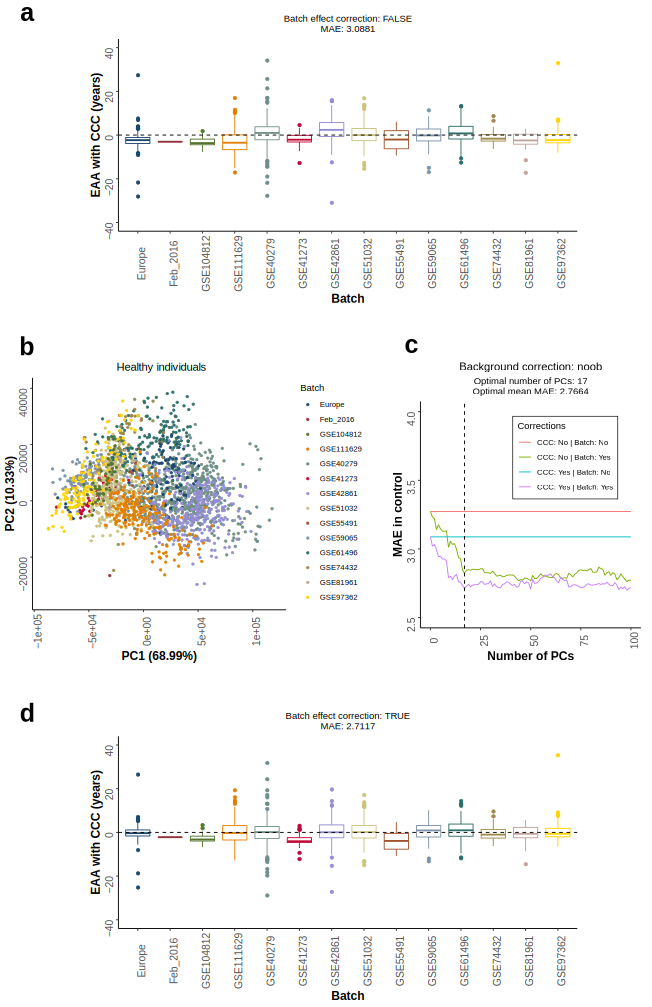
\includegraphics[width=0.8\textwidth]{C2_Fig13}
	\vspace*{2mm}    
	\caption[Correcting for batch effects in the context of the epigenetic clock]{Correcting for batch effects in the context of the epigenetic clock. \textbf{a.} Distribution of the epigenetic age acceleration (EAA) for the different batches of healthy individual samples, using the control model with cell composition correction (CCC) and before applying batch effect correction. The dashed black line represents $EAA = 0$, where the distributions should be centred around. \textbf{b.} Scatterplot showing the values of the first two principal components (PCs) for the healthy individual samples after performing PCA on the control probes of the 450K arrays. Each point corresponds to a different sample and the colours represent the different batches. The different batches cluster together in the PCA space, showing that the control probes indeed capture technical variation. Please note that all the PCA calculations were done using samples from both healthy individuals (full lifespan, $N=2218$) and cases from developmental disorders ($N=666$, see Chapter~\ref{c:3}). \textbf{c.} Plot showing how the median absolute error (MAE) of the prediction in the healthy individual samples, that should tend to zero, is reduced when the PCs capturing the technical variation are included as part of the modelling strategy (see equations \ref{eq:2.16} and \ref{eq:2.17}). The dashed line represents the optimal number of PCs (17) that was finally used. The optimal mean MAE is calculated as the average MAE between the green and purple lines. \textbf{d.} As in a., but after applying batch effect correction (i.e. equivalent to equation \ref{eq:2.16}).}
	\label{fig:c2_fig13}
\end{figure}

\bigskip

Finally, deviations from a median EAA close to zero in some of the batches after batch effect correction (Fig.~\ref{fig:c2_fig13}d, Fig.~\ref{fig:sc2_fig8}b) could be explained by other variables, such as a small batch size or an overrepresentation of young samples (Fig.~\ref{fig:c2_fig14}). The latter is a consequence of the fact that Horvath’s model underestimates the epigenetic ages of older samples, which I have discussed in the previous section. Thus, I have shown that correcting for batch effects in the context of the epigenetic clock is important, especially when combining datasets from different sources for meta-analysis purposes. Batch effect correction is essential to \textbf{remove technical variance that could affect the epigenetic age of the samples} and confound biological interpretation. Furthermore, given the flexibility of this modelling approach, I have applied batch effect correction across other types of analyses in the thesis, such as DMPs identification (see equation \ref{eq:2.10}).

\begin{figure}[htbp!] 
	\centering
	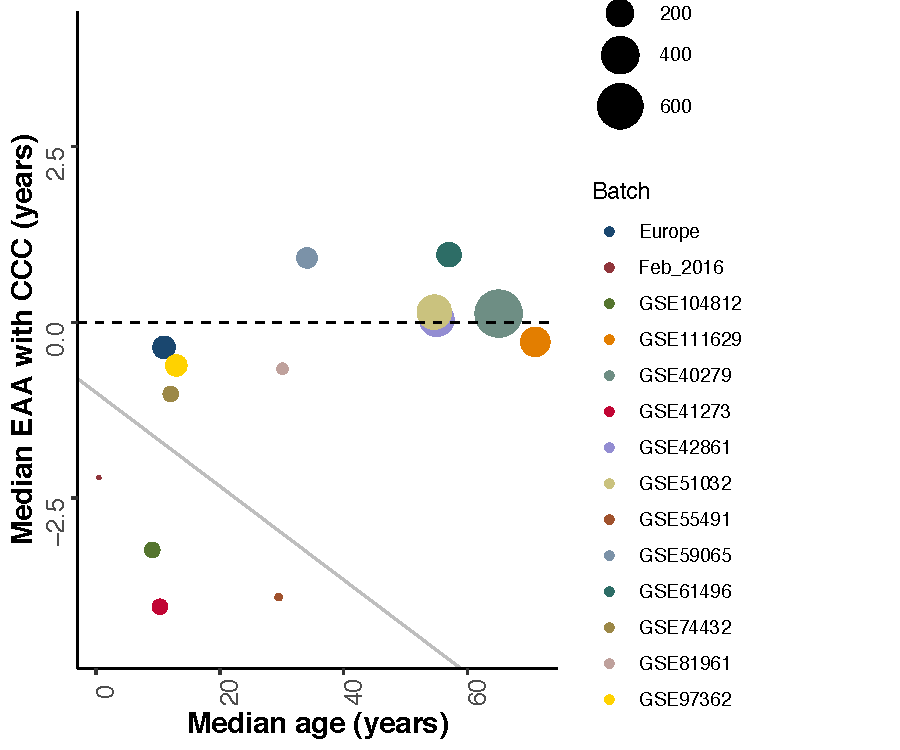
\includegraphics[width=0.7\textwidth]{C2_Fig14}
	\vspace*{2mm}    
	\caption[Causes of deviation from the expected EAA distribution in the control model]{After applying batch effect correction in the samples from the healthy individuals, deviations from a median epigenetic age acceleration (EAA) of zero (dotted black line) in some of the batches can be explained by other causes. The grey line separates in the lower left corner those weird batches (Feb\_2016, GSE104812, GSE41273, GSE55491), which have a small sample size and/or a low median age.}
	\label{fig:c2_fig14}
\end{figure}


\section{Behaviour of other epigenetic clocks during ageing}

\smallskip

\subsection{Hannum's epigenetic clock}

Besides Horvath's epigenetic clock, other models have been proposed in the literature to measure the ageing process using DNA methylation. Among them, Hannum's epigenetic clock has also been shown to accurately predict epigenetic age in several cohorts \citep{Chen2016,Marioni2015,Horvath2016,Marioni2018,Perna2016,Irvin2018}. Hannum's model was originally trained in whole blood and it makes use of a linear combination of $\beta$-values from 71 probes in the 450K array. 

\bigskip

I calculated the epigenetic ages according to Hannum's model ($HannumAge$), although I only used 68 out of the 71 probes (the other 3 were filtered out during my pre-processing). Hannum's epigenetic clock \textbf{performed quite accurately in the dataset of healthy individuals, although with a slight overestimation of the epigenetic ages} (Fig~\ref{fig:c2_fig15}a), which has also been previously observed \citep{Marioni2015}. Furthermore, it is possible to observe the non-linear behaviour of Hannum's clock for young ages ($\leq$ 20 years), for which the authors did not correct in their original publication \citep{Hannum2013}. Horvath's and Hannum's epigenetic clocks are correlated (Fig.~\ref{fig:c2_fig15}b). The magnitude of this correlation ($HannumAge$ vs $DNAmAge$: $\text{PCC} = 0.9778$) was slightly stronger than the correlation between $HannumAge$ and chronological age ($\text{PCC} = 0.9756$), which could highlight the fact that both models indeed  measure epigenetic age.

\bigskip

Next, I estimated the epigenetic age acceleration (EAA) according to Hannum's epigenetic clock, using similar models to the ones previously described (although in this case the dependent variable was $HannumAge$, see equations \ref{eq:2.16} and \ref{eq:2.17}). The median absolute errors for Hannum's model ($MAE_{\text{with CCC}} = 2.8422$ years, $MAE_{\text{without CCC}} = 2.9484$ years) were slightly higher than the ones obtained for Horvath's clock ($MAE_{\text{with CCC}} = 2.7117$ years, $MAE_{\text{without CCC}} = 2.8211$ years), which could also be influenced by the fact that three of the model probes were not available. The EAAs estimated by Hannum's and Horvath's clocks showed a moderate correlation (Fig.~\ref{fig:c2_fig15}c,d), consistent with previous estimates \citep{Irvin2018}. Including cell composition correction improved the correlation between the EAAs from both clocks, highlighting the fact that Hannum's clock seems to be confounded with the changes in blood cell composition with age \citep{Marioni2015,Irvin2018}. 

\bigskip

Overall, Hannum's epigenetic clock performed well in my dataset. However, given that it produces slightly worse predictions than Horvath's and could be partially tracking blood immunosenescence instead of multi-tissue ageing effects, I used the latter as my main proxy to measure the ageing process in this thesis. Finally, it is also worth mentioning that the data that was used to train Hannum's model (GSE40279) is also part of the dataset of healthy individuals that I assembled and, therefore, this analysis does not constitute a completely independent assessment of the behaviour of Hannum's epigenetic clock.


\begin{figure}[htbp!] 
	\centering
	\includegraphics[width=1\textwidth]{C2_Fig15}
	\vspace*{2mm}    
	\caption[Behaviour of Hannum's epigenetic clock in the healthy individuals]{Behaviour of Hannum's epigenetic clock in the healthy individuals. \textbf{a.} Scatterplot showing the relationship between the epigenetic age predicted with Hannum's model ($HannumAge$) \citep{Hannum2013} and chronological age of the samples for the healthy individuals. Each sample is represented by one point. The black dashed line represents the diagonal to aid visualisation. The solid brown line represents the linear model HannumAge $\sim$ Age. \textbf{b.} Relationship between the Hannum and Horvath epigenetic ages estimated for the same sample. The solid brown line represents the linear model HannumAge $\sim$ DNAmAge. \textbf{c.} Relationship between the epigenetic age acceleration (EAA) calculated with the Hannum and the Horvath's epigenetic clocks. In this case the models include cell composition correction (CCC). The solid brown line represents the linear model Hannum\_EAA$_{\text{with CCC}}$ $\sim$ Horvath\_EAA$_{\text{with CCC}}$. \textbf{d.} As in c., but in this case the models do not include CCC.}
	\label{fig:c2_fig15}
\end{figure}



\subsection{Epigenetic mitotic clock: \textit{epiTOC}} \label{s:2.3.2}

In 2016, Yang and colleagues conceived a novel type of epigenetic clock called \textit{\acrshort{epiTOC}} (epigenetic Timer Of Cancer), which measures the rate of (stem) cell division in both normal and cancerous tissues and is associated with cancer risk \citep{Yang2016}. This epigenetic mitotic clock tracks the gain in methylation levels that happens in 385 CpG sites, which localise in the promoter of genes that are targeted by Polycomb Repressing Complex 2 (\acrshort{PRC2}). Importantly, these CpG sites are unmethylated across fetal tissues and therefore this provides a ground state to measure these changes during human lifespan.

\bigskip

I calculated the mitotic age ($\acrshort{pcgtAge}$) of the healthy individuals in my dataset, although I only used 378 out of the 385 probes (the other 7 were filtered out during my pre-processing). The mitotic age of the individuals correlated with both chronological age (PCC $= 0.5131$, Fig.~\ref{fig:c2_fig16}a) and $DNAmAge$ (PCC $= 0.5602$, Fig.~\ref{fig:c2_fig16}b), which is expected given the cumulative number of divisions of the hematopoietic stem cells \citep{Beerman2013}. Furthermore, I estimated the epigenetic age acceleration (EAA) according to the epigenetic mitotic clock, using similar models to the ones previously described (although in this case the dependent variable was $pcgtAge$, see equations \ref{eq:2.16} and \ref{eq:2.17}). Interestingly, the EAAs for $pcgtAge$ and $DNAmAge$ showed a small but highly statistically significant correlation (Fig.~\ref{fig:c2_fig16}c,d). Moreover, I also did some preliminary work where I calculated the $DNAmAge$ of different healthy tissues (that came from cancer patients). I observed that tissues with a high turnover (such as breast) \citep{Horvath2013,Sehl2017} had a higher $DNAmAge$ when compared with tissues with a low turnover (data not shown). This was quite surprising given that Horvath's epigenetic clock predicts across tissues with different turnover rates \citep{Yang2016}. Additionally, it has been recently demonstrated that $DNAmAge$ increases linearly with cell passage \textit{in vitro} if TERT (the catalytic subunit of telomerase) is expressed (although whether this also applies \textit{in vivo} is unknown) \citep{Lu2018}. 

\bigskip

All of this, together with the fact that $DNAmAge$ has a stronger correlation with $pcgtAge$ than chronological age (at least in this blood dataset), could suggest that \textbf{Horvath's epigenetic clock might track cell division to a certain extent} (although it is also clear that Horvath's clock is mostly not a mitotic clock). Furthermore, it is important to point out that the observed effect sizes are small, that some of these results could be confounded by variables that are difficult to account for (e.g. higher $DNAmAge$ in breast tissue could be due to hormonal factors) and that $DNAmAge$ is not universally accelerated in cancer \citep{Horvath2015e}. Therefore, further testing of these ideas is required by future studies, which hopefully will improve our understanding of the contribution of cell division to Horvath's epigenetic clock and its relation to the hypermethylation in PRC2-bound regions as measured by the epigenetic mitotic clock.    


\begin{figure}[htbp!] 
	\centering
	\includegraphics[width=1\textwidth]{C2_Fig16}
	\vspace*{2mm}    
	\caption[Behaviour of the epigenetic mitotic clock ($epiTOC$) in the healthy individuals]{Behaviour of the epigenetic mitotic clock ($epiTOC$) in the healthy individuals. \textbf{a.} Scatterplot showing the relationship between mitotic age ($pcgtAge$) \citep{Yang2016} and chronological age of the samples for the healthy individuals. Each sample is represented by one point. The solid brown line represents the linear model pcgtAge $\sim$ Age. \textbf{b.} Relationship between $pcgtAge$ and $DNAmAge$ estimated for the same sample. The solid brown line represents the linear model pcgtAge $\sim$ DNAmAge. \textbf{c.} Relationship between the epigenetic age acceleration (EAA) calculated with the mitotic and the Horvath's epigenetic clocks. In this case the models include cell composition correction (CCC). The solid brown line represents the linear model pcgtAge\_EAA$_{\text{with CCC}}$ $\sim$ Horvath\_EAA$_{\text{with CCC}}$. \textbf{d.} As in c., but in this case the models do not include CCC.}
	\label{fig:c2_fig16}
\end{figure}


\section{Additional methods} \label{s:2.4}

\subsection*{A short introduction to the linear regression framework}

Linear models are a broad class of statistical analyses that are at the core of many bioinformatic methods, including differential RNA expression analyses \citep{Ritchie2015} or genome-wide association studies (GWAS) \citep{Visscher2017}. An instance of such models is linear regression \citep{Eaton2007}, a statistical approach that allows modelling of the relationship between:

\begin{itemize}
	
	\item A dependent variable $\mathbb Y$, with observations $y_i \in R$ and $i \in \{1, ..., n\}$, where $n$ is the total number of observations (i.e. samples). 
	
	\item One or more independent variables $\mathbb X_j$, with observations $x_{ij} \in R$ and $j \in \{1, ..., k\}$, where $k$ is the total number of independent variables (a.k.a covariates). These variables can indicate, for example, whether a specific condition or phenotype is present in a given sample, quantify the effects of a continuous variable (such as chronological age) or adjust for the effects of batch effects; which gives this statistical framework a great analytical flexibility \citep{Ritchie2015}.
	
\end{itemize}

We can describe the dependent variable $\mathbb Y$ as a function of the independent variables $\mathbb X_j$:

\begin{align}
y_i = \sum_{j=1}^{k} x_{ij}\beta_j + \epsilon_i
\end{align} 

where $\beta_j$ are unknown parameters that need to be estimated from the data and $\epsilon_i$ is the random error. In matrix form:

\begin{align}
\mathbf{y} = \mathbf{X}\mathbf{\beta} + \mathbf{\epsilon}
\end{align}

where  $\mathbf{y} \in R^n$ is the vector $\{y_1, ..., y_n\}$, $\mathbf{X} \in R^{n \times k}$ is the $n \times k$ matrix of $x_{ij}$'s, $\mathbf{\beta} \in R^k$ is the vector $\{\beta_1, ..., \beta_k\}$ and $\mathbf{\epsilon} \in R^n$ is the vector $\{\epsilon_1, ..., \epsilon_n\}$.

\bigskip

Assuming that $\mathbb E(\epsilon)=0$, Var$(\epsilon)=\sigma^2 > 0$ and Cov$(\epsilon)= \sigma^2\mathbf{I_n}$ (where $\mathbf{I_n}$ is the $n \times n$ identity matrix) and applying the Gauss-Markov theorem \citep{Eaton2007}, it can be demonstrated that:

\begin{align}
\mathbf{\hat{\beta}} = (\mathbf{X'}\mathbf{X})^{-1}\mathbf{X'}\mathbf{y}
\end{align}

where $\mathbf{X'}$ is the transpose of $\mathbf{X}$ and $\mathbf{\hat{\beta}}$ is the least-squares estimator of $\mathbf{\beta}$, since it minimises:

\begin{align}
\sum_{i=1}^{n} (y_i - \sum_{j=1}^{k} x_{ij}\hat{\beta}_j)^2
\end{align}

It is possible to test whether there is a statistically-significant linear association between the dependent variable ($\mathbb Y$) and one of the independent variables ($\mathbb X_j$) i.e. to test:

\begin{align}
H_0: \beta_j = 0 \quad \text{against} \quad H_A: \beta_j \ne 0
\end{align}
 
where $H_0$ is the null hypothesis and $H_A$ is the alternative hypothesis. A $t$-statistic ($T$) can be derived after performing the fitting of the linear regression model \citep{Sheather2009}:

\begin{align}
T=\frac{\hat{\beta}_j}{se(\hat{\beta}_j)} 
\end{align}

where $se(\hat{\beta}_j)$ is the standard error of $\hat{\beta}_j$. When $H_0$ is true, then the statistic $T$ follows a Student's $t$ distribution with $n-k$ degrees of freedom i.e. $T\sim t_{n-k}$. This allows to estimate the p-value for the linear association of $\mathbb Y$ with a given $\mathbb X_j$.

\bigskip

Finally, it is worth mentioning the nomenclature that I used for the linear regression models along this thesis. For example, the following model fits a linear association between the dependent variable (e.g. $\beta$-value at a specific CpG probe in the array) with intercept and 3 covariates (e.g. age, sex and disease status):

\begin{align}
\begin{bmatrix}
y_{1} \\
y_{2} \\
... \\
y_{n} \\
\end{bmatrix}
=
\begin{bmatrix}
1 & x_{11}  & x_{12} & x_{13} \\
1 & x_{21} & x_{22} & x_{23} \\
... & ... & ... & ... \\
1& x_{n1} & x_{n2} & x_{n3}  \\
\end{bmatrix}
%
\begin{bmatrix}
\beta_{0} \\
\beta_{1} \\
\beta_{2} \\
\beta_{3} \\
\end{bmatrix}
+
\begin{bmatrix}
\epsilon_{1} \\
\epsilon_{2} \\
... \\
\epsilon_{n} \\
\end{bmatrix}
\end{align}

where $y_i$ is the $\beta$-value at a certain CpG probe for the $i$th sample, $x_{i1}$ is the age for the $i$th sample, $x_{i2}$ is the sex (e.g. 0 for male and 1 for female) for the $i$th sample, $x_{i3}$ is the disease status (e.g. 0 for a healthy individual and 1 for an individual with a disease) for the $i$th sample, $\beta_0$ is the intercept coefficient, $\beta_j$ are the covariate coefficients ($j=1$ for age, $j=2$ for sex, $j=3$ for disease status) and $\epsilon_i$ is the error for the $i$th sample. 

\bigskip

Throughout this thesis, I use the following nomenclature to describe the model above (`R-style' nomenclature):

\begin{align}
\text{Beta} \sim \text{Age}+\text{Sex}+\text{Disease\_status}
\end{align}



